\documentclass[12pt]{article}
\usepackage{amsmath,amssymb}
\usepackage[dvipdfmx]{graphicx}
\topmargin=-45pt  \headheight=12truept \headsep=25pt
\footskip=37pt \hoffset=0pt \voffset=12pt
\oddsidemargin=0cm \evensidemargin=0cm
\textheight=23.7cm \textwidth=16.0cm

\def \nequiv {\equiv \hspace{-3mm} / \hspace{1mm}}
\def \qed {\hfill \hbox {\rule [-2pt]{3pt}{6pt}}}
%\pagestyle{myheadings}
%%%%%%%%%%%%%
\newtheorem{thm}{Theorem}%[chapter]% THEOREM
\newtheorem{theorem}[thm]{Theorem}
\newtheorem{prop}[thm]{Proposition}% PROPOSITION
\newtheorem{proposition}[thm]{Proposition}
\newtheorem{cor}[thm]{Corollary}% COROLLARY
\newtheorem{corollary}[thm]{Corollary}
\newtheorem{lem}[thm]{Lemma}% LEMMA
\newtheorem{lemma}[thm]{Lemma}
\newtheorem{remark}[thm]{Remark}
\newtheorem{defi}[thm]{Definition}
\newtheorem{definition}[thm]{Definition}
%\newtheorem{example}[thm]{Example}

\begin{document}
\title{Implicit American Monte Carlo Method for Semi Linear Financial Problem}
 
\author{
Yusuke MORIMOTO
\thanks{
Graduate School of Mathematical Sciences, 
The University of Tokyo, 
Komaba 3-8-1, Meguro-ku, Tokyo 153-8914, Japan, \
Bank of Tokyo Mitsubishi UFJ }
}
\date{}

\maketitle
\begin{abstract}
\end{abstract}

JEL classification:C63, G12

Mathematical Subject Classification(2010)   65C05,  60G40

Keywords:  computational finance, option pricing, Malliavin calculus, 
stochastic mesh method, XVA

Short (running) title stochastic mesh method

\section{Introduction}

In various situation in financial practice, calculation of following type of semi-linear expectation for a portfolio is necessary.
\begin{align}\label{eq:C0}
  C_0 = E^{\mu}\left[\int_{0}^T \left\{V(t) \vee0 \right \} \ dt \right],
\end{align}
where $(\Omega, \mathcal{F}, \{\mathcal{F}_t\}_{t\in [0,T]}, \mu)$ is filtered probability space, $V(t)$ is the portfolio value of future date $t$, and $T$ is risk horizon date.\\
In case that portfolio is composed of Eurean derivatives, $V(t)$ is expressed as
\begin{align}\label{eq:V}
  V(t) =  E^{\mu} \left[ \sum_{k:T_k\geqq t}F_k\left({X}(T_k)\right) |\mathcal{F}_t \right],
\end{align}
where $X$ is underlying stochastic process and $\{F_k\}$ are deterministic functions corresponding to the pay offs of European derivatives in the portfolio.

To calculate $C_0$, we needs a lot of computational resources for the following reasons.
\begin{enumerate}
  \item Monte Carlo simulation is often used for the general computation framework which can compute various type products contained in the portfolio.
  \item Dimension of $X$ is large when there are a lot of assets in the portflio.
  \item The path of $X$ should be generated at the same time for all products in the portfolio
    due to the non-linearity in te equation (\ref{eq:C0}).
  \item Conditonal expectation of equation $(\ref{eq:V})$ is needed for all $t \in [0, t]$,
    and using naive calculation, monte of monte simulation is needed.
\end{enumerate}

To deal with the last problem, American Monte carlo method is often used (see \cite{G}).
In the American Monte Carlo method, $V(t)$ is approximated by $\tilde{V}(t)$ which is rough but low computational cost estimation instead of naive monte carlo estimation.
We obtaion approximation of $C_0$ by substituting $V(t)$ by $\tilde{V}(t)$.
We call it "expicit method" which is denoted by $C_{\text{explicit}}$
\begin{align}
C_{\text{explicit}}=E^{\mu}\left[\int_{0}^T \left\{\tilde{V}(t) \vee0 \right \} \ dt \right].
\end{align}
On the other hand, we have the other expression of $C_0$ as follows.
\begin{align}\label{eq:implicit}
  C_0 &= E^{\mu}\left[\int_{0}^T \left\{ \sum_{k:T_k\geqq t} E^{\mu} \left[ F_k({X}(T_k)) |\mathcal{F}_t \right]\right \} 1_{\{V(t) \geqq 0\}}\ dt \right]\nonumber \\
      &=E^{\mu}\left[\int_{0}^T \left\{ \sum_{k:T_k\geqq t} F_k({X}(T_k)) 1_{\{V(t) \geqq 0\}}\right \} \ dt \right].
\end{align}
In this expression $V(t)$ is appeared only in the indicator function. Then only the sign of
$V(t)$ affects for the approximation accracy. In other words, how large the the difference between
$\tilde{V}$ and $V$ exists, there is no approximation error as long as the sign of $V$ and $\tilde{V}$are the same.
We call approximation by using equation(\ref{eq:implicit}) as "Implicit method" which is denoted by $C_{\text{implicit}}$.
\begin{align}
   C_{\text{implicit}}=E^{\mu}\left[\int_{0}^T \left\{ \sum_{k:T_k\geqq t} F_k({X}(T_k)) 1_{\{V(t) \geqq 0\}}\right \} \ dt \right].
\end{align}
In this paper we show two algorithms of approximation of $C_0$ based on "explicit method" and 
"implicit method" and obtain the error estimation which includes both Monte Carlo error and
discretization error.
There are mainly two types of method in American Monte Carlo method, Least Square Monte Carlo method and Stochastic mesh method (see \cite{G}, \cite{BG1}).
Least square monte carlo is more popular in plactice for its general algorithm and
less computational cost.
On the other hand, although it is only applicable to underlying path whose transition density function is  explicitly known, stochastic mesh method has accurate estimation(see \cite{KM}).
In this paper, we use stochastic mesh method for this reasons.

With regard to the meaning of $C_0$
For example CVA is expressed by 

$$\text{CVA}= E^Q[L(\tau)D(0,\tau)1_{\{\tau <T\}}V_0(\tau)_{+}]$$ $$=E^{Q}[\int_0^T L(t)D(0,t) V_0(t)_{+} \lambda(t) dt ]  .$$
where $$V_0(t) = \sum_{k:T_k\geqq t} E^{Q}[D(t,T) f_k(X^{(k)}) |\mathcal{F}_t].$$
 

 where $X=(X^{(1)}, \ldots, X^{(K)})$ be underlying multi assets process. $f_k, k=1,\ldots K$ be the pay off of derivative contract between one counter party. Let $Q$ be a 

 In this paper, we assume that there exists a state process $X^{(0)}$ such that $D(t,T), \lambda(t),
L(t)$ is represented by $X^{(0)}$, and payoff at $T_k$ depend on only $X^{(0)}$ and small number of 
assets $X^{(k)}$l, where $X=(X^{(1)}, \ldots, X^{(K)})$.



\section{Main Result}
\subsection{Setting}
Let $(\hat{\Omega}, \hat{\mathcal{F}}, Q, \{\mathcal{F}_t\}_{t\geqq 0})$ be a filtered probability space.
Let $N, d \geqq 1.$
Let $B^i:[0,\infty )\times \hat{\Omega} \to {\bf R},$ $i=1,\ldots ,d,$ be given 
by
$B^i(t,w) =w^i(t),$ $(t,w)\in [0,\infty )\times W_0.$
Then $ \{ (B^1(t), \ldots ,B^d(t) ; t \in [0,\infty ) \}$ 
is a $d$-dimensional Brownian motion.
Let $B^0(t) = t,$ $t \in [0,\infty ).$
Let $V_0,V_1,\ldots ,V_d$ 
$ \in C^{\infty}_b({\bf R}^N;{\bf R}^N).$
Here $C^{\infty}_b({\bf R}^N;{\bf R}^n)$ denotes 
the space of ${\bf R}^n$-valued smooth functions defined 
in ${\bf R}^N$ whose derivatives of any order are bounded.
We regard elements in $C^{\infty}_b({\bf R}^N;{\bf R}^N)$ 
as vector fields on ${\bf R}^N.$

Let $K \geqq 1$ be fixed, ${N}_k, d_k \geqq 1, k=1, \cdots, K$, 
$N= N_0+ \cdots + N_K$, $d=d_0+\cdots +d_K$, 
$ \tilde{N}_k=N_0+N_k$ and $\tilde{d}_k=d_0+d_k$.\\
Let we define a projection $\pi_k: {\bf R}^N \to {\bf R}^{\tilde{N}_k}, k=1,\ldots,K,$ as 
$$ \pi^{(k)}(x)= \tilde{x}_k, \quad k=1,\ldots,K,$$
where $x=(x_0,x_1, \cdots, x_K)$, $\tilde{x}_k=(x_0,x_k)$, and $x_i \in {\bf R}^{N_k}, i=1,\ldots,K$.\\
Then we also assume that $\pi_k(X(t,x))$  is represented as the solution of Stochastic differential equation
under the following setting.

Let $\mathcal{I} = \{(k,i); 1 \leqq k \leqq K , 1 \leqq i \leqq d_k \}$, $B^{k,i}:[0,\infty )\times W_0 \to {\bf R},$ $(k,i) \in \mathcal{I}$ be given 
by $B^{k, i}(t,w) =w^{k, i}(t),$ $(t,w)\in [0,\infty )\times W_0.$
Then $\{B^{k,i}(t); t \in [0,\infty ), (k,i)\in \mathcal{I} \}$ 
is a $d$-dimensional Brownian motions such that
$$d\langle B^{k, i}, B^{l, j} \rangle(t) = \rho_{k, i}^{l,j}dt,$$
where $ \rho_{k,i}^{l,j}: \mathcal{I} \times \mathcal{I} \to [-1,1] $ is a positive definite matrix. We further assume that
\begin{align*}
&\rho_{i, j}^{k,l}(t) = \delta_{i,j}, \quad k =l,\\
&\rho_{i, j}^{k,l}(t) =  0, \quad k\neq l, k=0 \ \text{or} \ l =0,
\end{align*}
where $\delta_{i,j}$ is Kronecker's delta.\\
We define filtration $\{\mathcal{F}_t\}_{0\leqq t \leqq T}$ as
$$\mathcal{F}_t= \sigma \{B^{k,i}(s); s \in [0,t], (k,i)\in \mathcal{I} \}.$$

\noindent Let $B^{k,0}(t) = t,$ $t \in [0,\infty ), k=0, \cdots, K.$
Let $V_{0, i}$ $ \in C^{\infty}_b({\bf R}^{{N}_0}; {\bf R}^{{N}_0}), i =0,\cdots, d_0,$
$V_{k, i} \in C^{\infty}_b({\bf R}^{{N}_0}\times {\bf R}^{{N}_k};{\bf R}^{{N}_k}), i =0, \cdots, d_k, k=1, \cdots, K.$
Here $C^{\infty}_b({\bf R}^{N} ;{\bf R}^{n})$ denotes 
the space of ${\bf R}^{n}$-valued smooth functions defined 
in ${\bf R}^{N}$ whose derivatives of any order are bounded.
We regard elements in $C^{\infty}_b({\bf R}^{N};{\bf R}^{N})$ 
as vector fields on ${\bf R}^N.$\\


\noindent Now let ${X}^{(0)}(t,{x}_0),$  ${x}_0\in {\bf R}^{{N}_0},$ 
${X}^{(k)}(t,{x}_k),$  ${x}_k\in {\bf R}^{{N}_k},$ 
be the solution to the Stratonovich stochastic integral equation 
\begin{equation}
{X}^{(0)}(t,x_0) = {x}_0 + \sum_{i=0}^{d_0} \int_{0}^{t} V_{0, i}({X}^{(0)}(s,{x}_0))\circ dB^{0, i}(s),
\label{eq:SDE0}
\end{equation}
\begin{equation}
{X}^{(k)}(t,x_k) = {x}_k + \sum_{i=0}^{d_k} \int_{0}^{t} V_{k, i}({X}^{(0)}(s,{x}_0), {X}^{(k)}(s,{x}_k))\circ dB^{k, i}(s).
\label{eq:SDEk}
\end{equation}
 To consider (\ref{eq:SDE0}) and (\ref{eq:SDEk}) together, we further prepare the following notation for each $k= 1,\ldots, K$.
 Let $\tilde{x}_k=(x_0, x_k), \pi_k{X}(t,\tilde{x}_k)=(X^{(0)}(t, x_0),X^{(k)}(t, x_k)), $
 \begin{align*}
 \tilde{B}^{k,i}(t)= 
 \begin{cases}
 B^{0,i}(t), \quad  0 \leqq i \leqq d_0, \\
 B^{k,i}(t), \quad d_0+1 \leqq i \leqq \tilde{d}_k.
 \end{cases}
 \end{align*}
 Let $\tilde{V}_{k, i} \in C^{\infty}_b({\bf R}^{{N}_0}\times {\bf R}^{{N}_k};{\bf R}^{{N}_0}\times{\bf R}^{{N}_k}), i =0, \cdots, \tilde{d}_k,$ be as follows.\\
 For $i=0$
 \begin{align*}
 \tilde{V}^j_{k,i}(x_0, x_k)= 
 \begin{cases}
  V^j_{0,0}(x_0), \quad  0 \leqq j \leqq N_0, \\
 V^j_{k,0}(x_0, x_k), \quad N_0+1 \leqq j \leqq \tilde{N}_k,\\
\end{cases}
 \end{align*}
for $ 1\leqq i \leqq d_0$
 \begin{align*}
 \tilde{V}^j_{k,i}(x_0, x_k)= 
 \begin{cases}
 V^j_{0,i}(x_0), \quad  0 \leqq j \leqq N_0, \\
 0, \quad  N_0+1 \leqq j \leqq \tilde{N}_k, \\
 \end{cases}
 \end{align*}
and for $ d_0+1 \leqq i \leqq \tilde{d}_k,$
  \begin{align*}
 \tilde{V}^j_{k,i}(x_0, x_k)= 
 \begin{cases}
0, \quad  N_0+1 \leqq j \leqq \tilde{N}_k, \\
 V^j_{k,i}(x_0, x_k), \quad N_0+1 \leqq j \leqq \tilde{N}_k.\\
 \end{cases}
 \end{align*}
Then (\ref{eq:SDE0}) and (\ref{eq:SDEk}) are written as 
\begin{align}
\pi_k{X}(t,\tilde{x}_k) = \tilde{x}_k + \sum_{i=0}^{\tilde{d}_k} \int_{0}^{t} \tilde{V}_{k, i}(\tilde{X}^{(0)}(s,\tilde{x}_0), \pi_k{X}(s,\tilde{x}_k))\circ d\tilde{B}^{k, i}(s).
\end{align}
Then there is a unique solution $\pi_k{X}(t,\tilde{x}_k)=({X}^{(0)}(t,{x}_0), {X}^{(k)}(t,{x}_k) )$ 
to this equation. Moreover we may assume that  $\pi_k{X}(t,\tilde{x}_k)$ 
is continuous in $t$ and smooth in $\tilde{x}_k$ 
and $\pi_k{X}(t,\cdot ):{\bf R}^{\tilde{N}_k}\to {\bf R}^{\tilde{N}_k}$ $t \in [0,\infty ),$
is a diffeomorphism with probability one.
\\

Let ${\cal A}_{k} =  \{ \emptyset \} \cup 
\bigcup_{j = 1}^{\infty} \{ 0,1,\ldots , \tilde{d}_k \}^j $ 
and for $\alpha \in {\cal A}_k$, 
let $|\alpha | = 0$  if  $\alpha = \emptyset ,$ 
let $|\alpha | = j$ if 
$\alpha $ $= (\alpha^1,\ldots ,\alpha^j)$
$\in \{ 0,1,\ldots , d_k \}^j ,$ and 
let $ \parallel \alpha \parallel $ 
$ = |\alpha | + \mbox{card}\{ 1 \leqq i \leqq |\alpha | ; 
\; \alpha^i = 0 \}.$ 
Let ${\cal A}_k^{*}$ and ${\cal A}_k^{**}$ denote 
${\cal A}_k\setminus \{ \emptyset \} $ and
${\cal A}_k\setminus \{ \emptyset , 0 \},$ respectively.
Also, for each $m\geqq 1,$ ${\cal A}^{**}_{k, \leqq m},$  
$\{ \alpha \in {\cal A}^{**}_k; \; \parallel \alpha \parallel \leqq m \} .$

We define vector fields $\tilde{V}_{k,[\alpha ]},$ $\alpha \in {\cal A},$ 
inductively by
$$
\tilde{V}_{k, [\emptyset ]} = 0, 
\qquad \tilde{V}_{k, [i]} = \tilde{V}_{k,i}, 
\quad i = 0,1,\ldots ,\tilde{d}_k,
$$
$$
\tilde{V}_{k, [\alpha *i]} = [\tilde{V}_{k, [\alpha ]},\tilde{V}_{k,i}], 
\qquad i = 0,1,\ldots ,\tilde{d}_k.
$$
Here $\alpha *i$ 
$= (\alpha^1,\ldots ,\alpha^j,i)$
for $\alpha $ $= (\alpha^1,\ldots ,\alpha^j)$ and $i = 0,1,\ldots ,\tilde{d}_k.$

We say that a system $\{ \tilde{V}_{k,i} ; i=0,1,\ldots ,\tilde{d}_k \}$ of vector fields 
satisfies the following condition (UFG).

\noindent
(UFG) There are an integer $\ell_k$ 
and $\varphi_{\alpha,\beta} \in C^{\infty}_b({\bf R}^{\tilde{N}_k}),$ 
$\alpha \in {\cal A}_k^{**},$ $\beta \in {\cal A}^{**}_{k, \leqq \ell_k},$ 
satisfying the following.
$$
{\displaystyle \tilde{V}_{k,[\alpha ]} 
= \sum_{\beta \in {\cal A}^{**}_{\leqq \ell_k}}
\varphi_{k, \alpha,\beta}\tilde{V}_{k,[\beta ]}},
\qquad 
\alpha \in {\cal A}_k^{**}.
$$
$$
{\displaystyle \tilde{V}_{k,[\alpha ]} 
= \sum_{\beta \in {\cal A}^{**}_{\leqq \ell_k}}
\varphi_{k, \alpha,\beta}\tilde{V}_{k,[\beta ]}},
\qquad 
\alpha \in {\cal A}_k^{**}, k=1,\ldots,K.
$$


Let $A_k(x)$ $= (A_k^{ij}(x))_{i,j=1,\ldots ,\tilde{N}_k},$ $t>0$ $x\in {\bf R}^{\tilde{N}_k}$ 
be a $\tilde{N}_k \times \tilde{N}_k$ symmetric matrix given by
$$
A_k^{ij}(x) 
= \sum_{\alpha \in {\cal A}^{**}_{k, \leqq \ell_k}}
\tilde{V}^i_{k,[\alpha ]}(x)\tilde{V}^j_{k,[\alpha ] }(x),
\qquad i,j=1,\ldots , \tilde{N}_k.
$$
Let $h_k(x) = \det A_k(x), x\in {\bf R}^{ \tilde{N}_k}$ 
and $E_k= \{ x\in {\bf R}^{\tilde{N}_k};\; h_k(x)>0\} .$
By \cite{KS2}, we see that if $x\in E_k,$ 
the distribution law of $\pi_k{X}(t,x)$ under $\mu$ has a smooth density function
$p^{(k)}(t,x,\cdot ):{\bf R}^{\tilde{N}_k}\to [0,\infty )$ for $t>0.$
Moreover, by \cite{KM} we see  that $\int_{E_k} p^{(k)}(t,x,y)dy =1,$ $x\in E_k.$ 
We have $p_k(t,x,y)=0, y\in E_k^c$ by \cite{KM}.\\
Let $\mathcal{L}(E_k)$ be the space of measurable functions on $E_k$ such that
for any $F\in \mathcal{L}(E_k)$ there exists a $g, h \in C^{\infty}({\bf R}^{N};{\bf R})$ and
$F=g\vee h$.

Let $\nu^{(k)}_t, t\geqq 0,$ be the probability law of $\pi_k{X}(t, \tilde{x}_k)$ under $\mu$.
Then we see that $\nu^{(k)}_0$ is the probability measure concentrated in $\tilde{x}_k$ and $\nu^{(k)}_t(dx)
=p^{(k)}(t,\tilde{x}_k, x)dx, t>0.$

For any $t>s\geqq 0,$ 
we can define a linear contraction map 
$P^{(k)}_{s,t}:L^1(E_k;d\nu^{(k)}_t)\to L^1(E_k;d\nu^{(k)}_s)$ by
$$
(P^{(k)}_{s,t}f)(x) = \int_{E_k} p^{(k)}(t-s,x,y)f(y) dy,
\qquad x \in E_k,\ f\in L^1(E_k;d\nu_t).
$$

Now let $X(t,x),$ $t\in [0,\infty ),$ $x\in {\bf R}^N,$ 
be the solution to the Stratonovich stochastic integral equation 
\begin{equation}
X(t,x) = x + \sum_{i=0}^{d} \int_{0}^{t} V_i(X(s,x))\circ dB^i(s).
\label{eq:SDE}
\end{equation}
Then there is a unique solution 
to this equation. 
Moreover we may assume that  $X(t,x)$ 
is continuous in $t$ and smooth in $x$ 
and $X(t,\cdot ):{\bf R}^N\to {\bf R}^N,$ $t \in [0,\infty ),$
is a diffeomorphism with probability one.

\subsection{Approximation of CVA}
In this paper, we consider how to approximate $c_0$.
\begin{align}
c_0 = E^{\mu}[\int_{0}^T \{( \sum_{k:T_k\geqq t} E^{\mu}[F_k(\pi_k{X}(T_k)) |\mathcal{F}_t])\vee0\}dt ]
\end{align}
Let 
$$\Delta = \{0=t_0 < t_1 < \ldots < t_n= T \}$$ be a subdivision of $[0,T]$, where $n(\Delta)$  be the number of descretization and $|\Delta| = \max{t_{i+1}-t_i}$. We assume that $\{T_k; k=1,\ldots,K\}$ are included in $\Delta$. Then we set
$$c_{\Delta}=\sum_{i=0}^{n-1}(t_{i+1}-t_i)E^{\mu}[\{\sum_{k; T_k \geqq t_{i+1}}^K(P_{T_k-t_i}^{(k)}F_k)(X^{(k)}(t_i,x))) \}\vee 0].
$$
When we denote the detail of subdivision as 
$$T_{k-1} = t_{i_{(k-1)}} < \ldots < t_{i_k-1} < t_{i_k}=T_k, k=1,\ldots,K,$$
then $c_{\Delta}$ is written as
$$
c_{\Delta}=\sum_{k=1}^K\sum_{i=i_{(k-1)}}^{{i_{k}}-1}(t_{i+1}-t_i) E^{\mu}[ \{\sum_{k'=k}^K(P_{T_k-t_i}^{(k')}F_{k'})(\pi_{k'} X(t_i,x))\}\vee0 ]
 $$

\subsection{Numerical Simulation Algorithm}
Let $(\Omega ,{\cal F},P)$ be a probability space,
and $X_{\ell }:[0,\infty )\times \Omega \to {\bf R}^N,$ 
$\ell =1,2,\ldots ,$ be continuous stochastic processes such that 
the probability laws on $C([0,\infty );{\bf R}^N)$ of
$X_{\ell}(\cdot )$ under $P$ and of $X(\cdot ,\tilde{x}_0)$ under $\mu$ 
are the same for all $\ell$ $=1,2,\ldots ,$ and that
$\sigma \{ X_{\ell}(t); \; t\geqq 0\},$ $\ell =1,2,\ldots ,$ are independent.\\

Let ${\cal F}_{t}^{(L)},$ $t\geqq 0,$ $L=0,1,\ldots , \infty $ be 
sub $\sigma$-algebra of ${\cal F}$ given by
$$
{\cal F}_{t}^{(L)} 
= \sigma \{ X_{\ell}(s); \; s\in [0,t], \ \ell =1,2,\ldots .L \},
$$
and
$$
{\cal F}_{t}^{(\infty )} 
= \sigma \{ X_{\ell}(s); \; s\in [0,t], \ \ell =1,2,\ldots \} .
\int_0^{\infty}f(x)dx.
$$
\\
Let $0 < T_1 < \cdots < T_K <T.$
We define a random linear operator (Stochastic mesh operator) $Q_{t,T_k,\varepsilon}^{(k)}, 0 \leqq t \leqq T, 0 < \varepsilon <\min_{1\leqq k \leqq K}(T_k-T_{k-1}),$ defined for $f \in \mathcal{L}(E_k)$ by
\begin{align*}
&(Q_{t,T_k,\varepsilon}^{(k,L,\omega)}f)(x)
=
\begin{cases}
\frac{1}{L} \sum_{l=1}^L \frac{f(X_l^{(k)}(T_k))p^{(k)}(T_k-t, x, \pi_k( X_l(T_k)))}{q_{t,T_k}^{(k,L,\omega)}(\pi_k (X_l(T_k)))}, 
\quad 0 \leqq t <T_k-\varepsilon ,\\
f(x), \quad T_k - \varepsilon \leqq t < T_k, \\
0, \quad T_k \leqq t \leqq T .
\end{cases}\\
&\text{where} \quad q_{t,T_k}^{(k,L,\omega)}(y)=\frac{1}{L}\sum_{l=1}^L p^{(k)}(T_k-t, \pi_k(X_{\ell}(t)), y).
\end{align*}

We will consider three algorithms as follows. All algorithm are based on the 
approximation of $P^{(k)}_{T-t}$ by Stochastic mesh operator $Q_{t,T,\varepsilon}^{(k)}$.\\

\noindent {\it Algorithm 1.}

\noindent \qquad[Step1] Generate independent paths 
$${\bf X}_1 = \{X_{\ell }(t); 0 \leqq t \leqq T, \ell =1,2,\ldots ,L\}$$
$${\bf X}_2=\{X^{'}_{m }(t); 0 \leqq t \leqq T,  m =1,2,\ldots ,M\}$$
\qquad[Step2]  For each path of ${\bf X}_2$ and each time grid $t_i$, we construct
$$(Q_{t_i,T_k,\varepsilon}^{(k,L,\omega)}F_k)(\pi_k(X^{'}_m(t_i))), \text{for every}\  k \  \text{such that} \ T_k > t_i ,$$
\qquad \qquad where $Q_{t,T,\varepsilon}^{(k,L,\omega)}$ is constructed by paths ${\bf X}_1$.

\noindent \qquad [Step3] Calculate
$$\tilde{c}_1=\frac{1}{M} \sum_{m=1}^M \sum_{i=0}^{n-1} (( \sum_{k:T_k\geqq t_{i+1}} (Q_{t_i,T_k,\varepsilon}^{(k,L,\omega)}F_k)(\pi_k(X^{'}_m(t_i))))\vee0)(t_{i+1}-t_i). $$

Although we generate the continuous paths in Step1, for the actual simulation, we use only values on the 
discrete time grids $\Delta_n$.

\noindent Algorithm1 is simple approximation such that  we substitute $P^{(k)}_{T_k-t} F_k$ by $Q_{t_i,T_k,\varepsilon}^{(k,L,\omega)}$.
On the other hand, notice the following equation,
\begin{align*}
&E^{\mu}[( \sum_{k:T_k\geqq t_{i+1}} E^{\mu}[F_k(\pi_k{X}(T_k)) |\mathcal{F}_t])\vee0]\\
=&E^{\mu}[( \sum_{k:T_k\geqq t_{i+1}} E^{\mu}[F_k(\pi_k{X}(T_k)) |\mathcal{F}_t])
 1_{\{\sum_{k:T_k\geqq t_{i+1}} (P^{(k)}_{T_k-t} F_k)(\pi_k{X}(t))) \geqq 0\}}]\\
=&E^{\mu}[ \{ \sum_{k:T_k\geqq t_{i+1}} F_k(\pi_k{X}(T_k))\}
 1_{\{\sum_{k:T_k\geqq t_{i+1}} (P^{(k)}_{T_k-t} F_k)(\pi_k{X}(t))) \geqq 0\}}].
\end{align*}
Based on this equation, we can consider the following algorithm.\\

\noindent {\it Algorithm 2.}

\noindent \qquad[Step1] Generate independent paths 
$${\bf X}_1 = \{X_{\ell }(t); 0 \leqq t \leqq T, \ell =1,2,\ldots ,L\}$$
$${\bf X}_2=\{X^{'}_{m }(t); 0 \leqq t \leqq T,  m =1,2,\ldots ,M\}$$
\qquad [Step2]  For each path of ${\bf X}_2$ and each time grid $t_i$, we construct
$$(Q_{t_i,T_k,\varepsilon}^{(k,L,\omega)}F_k)(\pi_k(X^{'}_m(t_i))), \text{for every}\  k \  \text{such that} \ T_k > t_i ,$$
\qquad where $Q_{t,T,\varepsilon}^{(k,L,\omega)}$ is constructed by paths ${\bf X}_1$.

\noindent \qquad [Step3] Calculate
$$\tilde{c}_2= \frac{1}{M} \sum_{m=1}^M \sum_{i=0}^{n-1} \{ \sum_{k:T_k\geqq t_{i+1}}F_k(X_m^{'(k)}(T_k))\}
 1_{\{\sum_{k:T_k\geqq t_{i+1}} (Q_{t,T,\varepsilon}^{(k,L,\omega)}F_k)(\pi_k(X^{'}_m(t_i)))) \geqq 0\}}(t_{i+1}-t_i).$$ 
 
 \noindent In this algorithm, we do not use the approximation $Q_{t,T,\varepsilon}^{(k,L,\omega)}$ explicitly.
 We use it only to judge whether $(P^{(k)}_{T_k-t} F_k)(\pi_k(X^{'}_m(t_i))))>0$ or not. 
 So the approximation has no error when the signs of  $(Q_{t,T,\varepsilon}^{(k,L,\omega)} F_k)(\pi_k{X}(t)))$ and $(P^{(k)}_{T_k-t} F_k)(\pi_k(X^{'}_m(t_i)))$ are the same, even if there is large difference between their values.

In Algorithm 1 and 2, we use two independent sets of paths as ${\bf X}_1$ and ${\bf X}_2$.
One paths are used for Monte-Carlo simulation and another paths are used to construct Stochastic mesh operator.
But we can use the same paths for Monte-Carlo simulation and construction  of Stochastic mesh operator \\

\noindent {\it Algorithm 3.}

\noindent \qquad [Step1] Generate independent paths 
$${\bf X}_1 = \{X_{\ell }(t); 0 \leqq t \leqq T, \ell =1,2,\ldots ,L\}$$

\noindent \qquad[Step2] For each path of ${\bf X}_2$ and each time grid $t_i$, we construct
$$(Q_{t_i,T_k,\varepsilon}^{(k,L,\omega)}F_k)(\pi_k(X_{\ell}(t_i))), \text{for every}\  k \  \text{such that} \ T_k > t_i ,$$
\qquad \qquad \qquad where $Q_{t,T,\varepsilon}^{(k,L,\omega)}$ is constructed by paths ${\bf X}_1$.

\noindent \qquad [Step3] Calculate
$$\tilde{c}_3=\frac{1}{L} \sum_{\ell=1}^L \sum_{i=0}^{n-1} (( \sum_{k:T_k\geqq t_{i+1}} (Q_{t_i,T_k,\varepsilon}^{(k,L,\omega)}F_k)(\pi_k(X_{\ell}(t_i)))\vee0)(t_{i+1}-t_i). $$

\subsection{Main Theorem}
Let  $C^q_b({\bf R}^n)$ be the the space q-times continuously differentiable functions such that
$$\frac{\partial^{|\alpha|}f}{\partial x^{\alpha}} < \infty, \text{for any}  f \in C^q_b({\bf R}^n), |\alpha| \leqq q.$$
Let $C_{Lip}({\bf R}^n)$, be the space of Lipshitz continuous functions and for $f\in C_{Lip}({\bf R}^n)$,
$$\|f\|_{C_{Lip}}=\sup_{x,y\in {\bf R}^n,
x \neq y} \frac{|f(x)-f(y)|}{|x-y|}.$$
Let $C_{Lip,q}({\bf R}^n), q\geqq 0$ be the linear subspace of $C_{Lip}({\bf R}^n)$  spanned by
$$\{f \vee g;  f, g \in C^q_b({\bf R}^n)\}.$$

Related to the Algorithm 1 to 3, we define 
$\hat{c}_i : \Omega \to {\bf R} , i=1,2,3$ as follows.
\begin{align*}
&\hat{c}_1(\omega) =E^{\mu} [ \sum_{i=0}^{n-1}(t_{i+1}-t_{i}) \{(\sum_{k:T_k\geqq t_{i+1}} (Q_{t_i,T_k,\varepsilon}^{(k,L,\omega)}F_k)(\pi_k{X}(t))\vee0\} ],\\
&\hat{c}_2(\omega)=\sum_{i=0}^{n-1}(t_{i+1}-t_{i}) E^{\mu}[( \sum_{k:T_k\geqq t_{i+1}}F_k(\pi_k X(T_k)))
 1_{\{\sum_{k:T_k\geqq t_{i+1}} (Q_{t_i,T_k,\varepsilon}^{(k,L,\omega)}F_k)(\pi_k X(t_i))) \geqq 0\}}]\\
&\hat{c}_3(\omega)=\frac{1}{L} \sum_{\ell=1}^L \sum_{i=0}^{n-1} (( \sum_{k:T_k\geqq t_{i+1}} (Q_{t_i,T_k,\varepsilon}^{(k,L,\omega)}F_k)(\pi_k(X_{\ell}(t_i)))\vee0)(t_{i+1}-t_i).
\end{align*}

To approximate $c_0$ by $\hat{c}_1$ and $\hat{c}_2$, we estimate the error between them in the following.
Let $\ell_0 = \max\{\ell_k; k=1,\ldots, K\}$ and $\tilde{N} = \max\{\tilde{N}_k; k=1,\ldots, K\}$.
\begin{theorem}\label{main1}
If $F_k \in C_{Lip,q}({\bf R}^{\tilde{N}_k}), k=1,\ldots,K.$ 
 There are $\Omega_{L} \in \mathcal{F}, L\geqq 1$ and $C_{p,\delta}>0$ such that $P(\Omega_{L}^c) \to 0, L\to \infty$
 and
\begin{align}
|\hat{c}_1(\omega)-c_0| \leqq C_{p,\delta}L^{-\frac{3/2(1-\delta)^2}{2+(1+\delta)(\tilde{N}+1)\ell_0/2}},
\end{align}
for any $\omega \in \Omega_{L}$ and $L \geqq 1$.
If there exists $\gamma \in (0,1]$ such that
$$\int_0^T E^{\mu}
[ 1_{| \sum_{k:T_k\geqq t_{i+1}} (P_{T_k-t}^{(k)}F_k)(\pi_k (X(t)))| \leqq \theta\} } ]dt =O(\theta^{\gamma})
 , \text{as} \ \theta \downarrow 0,$$
\begin{align}
|\hat{c}_2(\omega)-c_0| \leqq C_{p,\delta}L^{-\frac{3(\gamma+1)(1-\delta)^2}{(\gamma+2)(2+(1+\delta)(\tilde{N}+1)\ell_0/2)}},\end{align}
\end{theorem}

\begin{remark}
Theorem \ref{main1} means that the estimation of $\hat{c}_2$ is better than $\hat{c}_1$. 
Especially if $\gamma = 1$, the convergence order for the number of paths  improves by $4/3$ times.
\end{remark}

\begin{remark}
Let $X_{m}^{'(k)}:[0,\infty ) \times \Omega \to {\bf R}^N_k,$ 
$m =1,2,\ldots ,$ be continuous stochastic processes, i.i.d with
$X_{l}(\cdot )$ $l$ $=1,2,\ldots$.
When we carry out the numerical simulation, we approximate $c_0$ by 
$$\hat{c}_1^{'}= \frac{1}{M} \sum_{m=1}^M \sum_{i=0}^{n-1} (( \sum_{k:T_k\geqq t_{i+1}} (Q_{t_i,T_k,\varepsilon}^{(k,L,\omega)}F_k)(X_m^{'(k)}(t_i)))\vee0)(t_{i+1}-t_i) ,$$ 
and
$$\hat{c}_2^{'}= \frac{1}{M} \sum_{m=1}^M \sum_{i=0}^{n-1} ( \sum_{k:T_k\geqq t_{i+1}}F_k(X_m^{'(k)}(T_k)))
 1_{\{\sum_{k:T_k\geqq t_{i+1}} (Q_{t,T,\varepsilon}^{(k,L,\omega)}F_k)(X_m^{'(k)}(t))) \geqq 0\}}(t_{i+1}-t_i),$$ 
 instead of $\hat{c}_1$ and $\hat{c}_2$.
 For simplicity we ignore the error from the difference between 
 expectation and monte-carlo simulation. 
\end{remark}

\begin{theorem} \label{main2}
If $\Delta_n\leqq C L^{-1/2}$
\begin{align*}
&E[|\hat{c}_3(\omega)-c_0|]
\leqq   C_{p,\delta}L^{-\frac{(1-\delta)^2}{1+(1+\delta)(\tilde{N}+1)\ell_0/2}},
\end{align*}
\end{theorem}

\section{Discretization}
Let the discretization $\Delta $ be
$$\Delta: 0=t_0 < t_1 < \ldots < t_n = T,$$
and let $c_{\Delta}$ be
$$c_{\Delta}=\sum_{i=0}^{n-1}(t_{i+1}-t_i)E^{\mu}[\{\sum_{k; T_k \geqq t_{i+1}}^K(P_{T_k-t_i}^{(k)}F_k)(X^{(k)}(t_i,x))) \}\vee 0].
$$
$$
=\sum_{k=1}^K\sum_{i=i_{(k-1)}}^{{i_{k}}-1}(t_{i+1}-t_i) E^{\mu}[ \{\sum_{k'=k}^K(P_{T_k-t_i}^{(k')}F_k')(\pi_k' X(t,x))\}\vee0 ]
 $$
Let $\varphi$ be a smooth function that satisfies
\begin{align*}
&\varphi(z)=
\begin{cases}
1 , z\geqq 1\\
0, z<0,
\end{cases}\\
&\varphi' (z) \geqq 0.
\end{align*}
Let $\varphi_m(z)=\varphi(mz)$ and $\bar{\varphi}$ be 
\begin{align*}
\bar{\varphi}_m(z)=\int_{0}^z \varphi_m(z')dz'.
\end{align*}
Then for any $z \in {\bf R},$
$$\bar{\varphi}_m(z) \to z \vee 0 , \quad m\to \infty.$$

Let $\mathcal{L}_0({\bf R}^N)$ be a class of functions such that 
$f \in C^{\infty}({\bf R}^{\tilde{N}}),\|\frac{\partial^{\alpha}f}{\partial x^{\alpha}}\|_{\infty} <\infty$ for any $|\alpha| \geqq 1.$
Let $\mathcal{L}_1({\bf R}^N)$ be a class of functions such as  linear combination of $f \vee g, f \wedge g$ etc.$f \in C^{\infty}({\bf R}^{\tilde{N}}),\|\frac{\partial^{\alpha}f}{\partial x^{\alpha}}\|_{\infty} <\infty$ for any $|\alpha| \geqq 1.$
where $\alpha=(\alpha_1,\ldots, \alpha_{\tilde{N}_k})\in {\bf Z}^{\tilde{N}_k}$ is multi index and $|\alpha|=\alpha_1+\ldots+ \alpha_{\tilde{N}_k}$.
Let $n, K \in {\bf N}, n> K$,  $\Delta_n: 0 = t_0 < t_1 < \cdots < t_n = T$ be time grids and 
$\mathcal{T}_{ex} = \{T_k, k=1,\ldots,K\}$ be a times of Payoff.
We set $|\Delta_n| = \max_{i=1,\ldots,n}(t_i-t_{i-1})$.We assume $\mathcal{T}_{ex} \subset \Delta_n$ and
$T_{k-1}=t_{i_{(k-1)}} <t_{i_{(k-1)}+1}  < \ldots < t_{i_{(k-1)}} <t_{i_{k}}=T_k, k=1,\ldots, K.$

\begin{lem}\label{discLem2}
Let $T>0, F \in \mathcal{L}_0({\bf R}^N)$ and we set $\{\mathcal{F}_t\}_{t\geqq 0}$-martingale $\{M_t\}_{t\geqq 0}$
as follows.
$$M_t = E^{\mu}[F(X(T,x))|\mathcal{F}_t]$$ 
$$=(P_{T-t}F)(X(t,x)).$$
Then for any $0< s < t< T$, there exists a $C>0$ such that 
$$|E[M_t \vee 0]-E[M_s \vee 0]|\leqq C \int_{s}^t(r^{-1/2}+(T-r)^{-1/2})dr .$$
\end{lem}
{\it Proof.}
By It\^o formula, 
$$\bar{\varphi}_m(M_t)=\bar{\varphi}_m(M_s)+\int_s^t\varphi_m(M_r)dM_r+\frac{1}{2}\int_s^t\varphi'_m(M_r)d\langle M \rangle_r$$
Now we set $$M_t=u(t,X(t,x)),$$ then
$$dM_t=\sum_{j=1}^d V_j u(t,X(t,x))dB^j(t)$$
$$d\langle M \rangle_t=\sum_{j=1}^d (V_j u(t,X(t,x)))^2dt.$$
So we have
$$E^{\mu}[\bar{\varphi}_m(M_t)]-E^{\mu}[\bar{\varphi}_m(M_s)]$$
$$=\frac{1}{2}\sum_{j=1}^d \int_s^t E^{\mu}[\varphi'_m( u(r,X(r,x)) ) (V_j u(r,X(r,x)))^2] dr.$$

On the other hand
$$ E^{\mu}[\varphi'_m( u(r,X(r,x)) ) (V_j u(r,X(r,x)))^2]$$
$$=E^{\mu}[V_j \varphi_m( u(r,X(r,x)) ) V_j u(r,X(r,x)] $$
$$=E^{\mu}[V_j\left( \varphi_m( u(r,\cdot) V_j u(r,\cdot)\right)(X(r,x))) - 
\varphi_m( u(r,X(r,x)) V_j^2 u(r,X(r,x)))] $$
$$=P_r  V_j  \varphi_m \left( ( P_{T-r}F)(\cdot) V_j P_{T-r}F (\cdot) \right)(x)- 
P_r \left ( \varphi_m \left( ( P_{T-r} F) (\cdot)\right)  V_j^2 (P_{T-r} F)(\cdot) \right)(x)$$
By Propostion \ref{rev}, there exists a $C_1 >0$ such that
$$\|P_r  V_j  \varphi_m \left( ( P_{T-r}F)(\cdot) V_j P_{T-r}F (\cdot) \right)\|_{\infty}) \leqq C_1(r^{-1/2}+(T-r)^{-1/2})$$
And with respect to another term, 
$$V_j^2 (P_{T-r} F)(x)=V_j \sum_{i=1}^N v_j^i(x) \frac{\partial}{\partial x_i}E[F(X(T-r,x))]$$
$$=V_j \sum_{i=1}^N v_j^i(x) E[\sum_{k=1}^N \frac{\partial F}{\partial x_k}(X(T-r,x)) \frac{\partial X^k(T-r,x)}{\partial x_i}]$$
$$=V_j \sum_{i=1}^N v_j^i(x) \sum_{k=1}^N T_{J_k^i} (T-r)\frac{\partial F}{\partial x_k} (x) .$$
Because $\|\frac{\partial F}{\partial x_k}\|_{\infty} < \infty, k=1,\cdots,N$ and $v_j^i \in C_0^{\infty},$ by Proposition \ref{rev},
there exists a $C_2 >0$ such that
$$ \|P_r \left ( \varphi_m \left( ( P_{T-r} F) (\cdot)\right)  V_j^2 (P_{T-r} F)(\cdot) \right)\|_{\infty} \leqq C_2 (T-r)^{1/2}.$$

So we can take a $C>0$ which is independent of $m$ and we have
$$E^{\mu}[\bar{\varphi}_m(M_t)]-E^{\mu}[\bar{\varphi}_m(M_s)]$$
$$\leqq C\int_{s}^t (r^{-1/2}+(T-r)^{-1/2})dr.$$
 \qed


\begin{prop}\label{time disc}
Let $F_k \in \mathcal{L}_1({\bf R}^{\tilde{N}_k}), k=1,\ldots,K$. there exists a $C >0$ such that
\begin{align}
&|\sum_{k'=1}^K\sum_{i=i_{k'-1}}^{{i_{k'}}-1}E^{\mu}[ \int_{t_i}^{t_{i+1}} \{\sum_{k=k'}^K(P_{T_k-t}^{(k)}F_k)(\pi_k X(t,x))\}\vee 0 dt] \nonumber\\
 -&\sum_{k'=1}^K\sum_{i=i_{k'-1}}^{{i_{k'}}-1}(t_{i+1}-t_i) E^{\mu}[ \{\sum_{k=k'}^K(P_{T_k-t_i}^{(k)}F_k)(\pi_k X(t,x))\}\vee0 ]|
 \leqq  C |\Delta|,
\end{align}
for any $0<s<t<T$.
\end{prop}
{\it Proof.}
Let $$F(x)=\sum_{k=k'}^K (P_{T_k-T_k'}^{(k)}F_k)(\pi_k x)$$
and $$\tilde{F_m}(x)=\psi_m * F_m$$ 
By Lemma \ref{discLem2}, the last term is bounded above by 
$$|E^{\mu}[ \int_{t_i}^{t_{i+1}} \{\sum_{k=k'}^K(P_{T_k-t}^{(k)}F_k)(\pi_k X(t,x))\}\vee 0 dt]-E^{\mu}[ \int_{t_i}^{t_{i+1}}  \{\sum_{k=k'}^K(P_{T_k-t_i}^{(k)}F_k)(\pi_k X(t_i,x))) \}\vee 0 dt]|$$
$$ \leqq \int_{t_i}^{t_{i+1}}dt \int_{t_i}^t (r^{-1/2}+(T_k-r)^{-1/2})dr.$$
So
$$\sum_{k;T_k\geqq t_{i+1}}  \sum_{i=0}^{n-1}\int_{t_i}^{t_{i+1}}dr \int_{r}^{t_{i+1}} (r^{-1/2}+(T_k-r)^{-1/2})dt $$
$$=\sum_{k;T_k\geqq t_{i+1}}  \sum_{i=0}^{n-1}\int_{t_i}^{t_{i+1}} (t_{i+1}-r) (r^{-1/2}+(T_k-r)^{-1/2})dr $$
$$\leqq |\Delta_n|\sum_{k;T_k\geqq t_{i+1}} \int_{T_{k-1}}^{T_{k}}  (r^{-1/2}+(T_k-r)^{-1/2})dr \leqq  C|\Delta_n|.$$
for some $C>0.$
As a result we have the assertion.
\qed


\section{Property of Stochastic Mesh Operator}
To estimate Stochastic mesh operator, we use the following estimation of 
transition kernel $p^{(k)}(t,\tilde{x}_k, x)$ obtained by Proposition 8 of  \cite{KM}.
\begin{proposition}\label{heatKernel}
Let $\delta_0^{(k)}$ be given by 
$$\delta_0^{(k)}=(3\tilde{N}_k(\sup_{x\in {\bf R}^{\tilde{N}_k}} \sum_{i=1}^{\tilde{d}_k}|\tilde{V}_{k,i}(x)|^2))^{-1},$$
then for any $T>0,$ there is a $C>0$ such that
$$
p^{(k)}(t,x,y)
\leqq C t^{- (\tilde{N}_k+1) \ell_k /2} h_k(x)^{-2(\tilde{N}_k+1)\ell_k}\exp (- \frac{2\delta_0^{(k)}}{t}|y-x|^2 ), 
\qquad  t \in (0,T], \ x,y \in E_k,
$$
and
$$
p^{(k)}(t,x,y)
\leqq C t^{- (\tilde{N}_k+1) \ell_k /2} h_k(y)^{-2(\tilde{N}_k+1)\ell_k}\exp (- \frac{2\delta_0^{(k)}}{t}|y-x|^2 ), 
\qquad  t \in (0,T], \ x,y \in E_k,
$$
for any $k=1,\ldots,K.$\\
In particular, for any $T>0$ and $m\geqq 1,$ 
there is a $C>0$ such that
$$
p^{(k)}(t,x,y)
\leqq C t^{- (\tilde{N}_k+1) \ell_k /2} h_k(x)^{-2(\tilde{N}_k+1)\ell_k}(1+|x|^2)^m
(1+|y|^2)^{-m}, 
\qquad  t \in (0,T], \ x,y \in E_k,
$$
for any $k=1,\ldots,K.$
\end{proposition}

By Proposition 13 and 21 of \cite{KM}, we have the followings.
\begin{proposition}\label{basic}
Let $t>s\geqq 0,$ 
and bounded measurable function $f:E_k\to {\bf R}.$
Then we have 
$$
E^P[(Q_{s,t}^{(k,L,\omega)}f)(x)| {\cal F}_{s}^{(\infty )}] 
= (P^{(k)}_{s,t}f)(x),
\qquad \nu_s^{(k)}-a.e.x.
$$
and 
$$
E^P[ |(Q_{s,t}^{(k,L,\omega)}f)(x) - (P^{(k)}_{s,t}f)(x)|^2 | {\cal F}_s^{(\infty )}]
\leqq 
\frac{1}{L}
\int_{E} \frac{p^{(k)}(t-s,x,y)^2 |f(y)|^2}{q_{s,t}^{(k,L,\omega)}(y)}\; dy .
$$
\end{proposition}

\begin{prop}\label{exSet}
We set
\begin{align*}
Z_L^{(k)}(t;\delta)=\sup_{y\in {\bf R}^{N_k}} \frac{|q_{t,T_k}^{(k,L,\omega)}(y)- p^{(k)}(T_k, x_0, y)|}
{(L^{-1/(1-\delta)}+p^{(k)}(T_k, x_0,y))^{(1-\delta)/2}},
\end{align*}
\begin{align*}
\tilde{Z}_L^{(k)}(t; \delta)=\sup_{s\in [0,t]} Z_L^{(k)}(s;\delta).
\end{align*}
Then, we have followings.\\
$(1)$ Let $\delta \in (0,1)$, then for any $p > 1$, there is a $C_{p,\delta} > 0$ such that
$$
E^P[(L^{(1-\delta^2)/2}\tilde{Z}_L(T_k-\varepsilon; \delta))^p]^{1/p}\leqq C_{p,\delta}\varepsilon^{-5l_0}L^{-p\delta^2/2+1/p},
\quad \varepsilon \in  (0,T].$$
$(2)$ Let $\delta \in (0,1), t \in (0, T)$ and $\varepsilon \in (0,T).$  If $L^{(1-\delta^2)/2}\tilde{Z}_L(t; \delta) \leqq 1/4$, and  $p^{(k)}(T_k, x_0, y) \geqq L^{-(1-\delta)}$, then
$$
\frac{1}{2} \leqq \frac{q_{t,T_k}^{(k,L,\omega)}(y)}{p^{(k)}(T_k, x_0, y)} \leqq 2,  \quad t \in (0, T_k-\varepsilon].
$$
\end{prop}

Now we prepare the following sets and functions.

Let $B^{(k)}(t, \delta)$, $\varphi_k(y)$ be 
$$
B^{(k)}(t, \delta) = \{\omega \in \Omega; L^{(1-\delta^2)/2}\tilde{Z}_L(t; \delta)
\leqq 1/4 \},
$$
$$
\varphi_k(y) = 1_{\{ y \in E_k; p^{(k)}(T_k, x_0, y) > L^{-(1-\delta)} \}},
$$
and let the measurable functions $ d_{1,\varepsilon}^{(k)}(t,x) , d_{2,\varepsilon}^{(k)}(t,x)  : [0,T] \times E \times \Omega \to [0, \infty)$ be as follows.
$$ d_{1,\varepsilon}^{(k)}(t,x) = |(Q_{t,T_k, \varepsilon}^{(k)}(1-\varphi_k)F_k)(x)
-(P_{T_k-t}^{(k)} (1-\varphi_k)F_k)(x) |,$$
$$ d_{2,\varepsilon}^{(k)}(t,x) = 1_{B^{(k)}(T_k-\varepsilon, \delta)}|(Q_{t,T_k, \varepsilon}^{(k)}\varphi_kF_k)(x)
-(P_{T_k-t}^{(k)} \varphi_kF_k)(x) |,$$
$\quad k = 1, \cdots, K.$

 We will estimate $d_{1,\varepsilon}^{(k)}$ and $d_{2,\varepsilon}^{(k)}$ in the next section.

\section{Estimation of  $d_{1,\varepsilon}^{(k)}$ and $d_{2,\varepsilon}^{(k)}$}
\begin{lem}\label{discLem1}
Let $0 < t < T, F_k \in \mathcal{L}_1({\bf R}^{N_k})$. Then there exists $C>0$ such that
\begin{align}
E^{\mu}[ |(P^{(k)}_{T-t}F_k)(\pi_k{X}(t,x))-F_k(\pi_k{X}(t,x))|] \leqq C(T-t), \quad k=1,\ldots,K.
\end{align}
\end{lem}
{\it Proof.}
By definition of $\mathcal{L}_k$, we can write $F_k=f_k\vee g_k = (f_k-g_k)\vee 0 +g_k,$ such that $\|\frac{\partial^{\alpha}f_k}{\partial x^{\alpha}}\|_{\infty} <\infty, \|\frac{\partial^{\alpha}g_k}{\partial x^{\alpha}}\|_{\infty} <\infty,  \text{for any } |\alpha| \geqq 1.$\\
By It\^o's formula we can easily prove that
$$E^{\mu}[ |(P^{(k)}_{T-t}g_k)(\pi_k{X}(t,x))-g_k(\pi_k{X}(t,x))|] \leqq C(T-t).$$
So it is sufficient to prove for $(f_k-g_k)\vee 0$ and we set $h=f_k-g_k.$\\
By It\^o's formula
$$\bar{\varphi}_m(h(\pi_k{X}(T,x))-\bar{\varphi}_m(h(\pi_k{X}(t,x))$$
$$=\int_t^T \varphi_m(h(\pi_k{X}(s,x)) \tilde{V}_{k,i}h(\pi_k{X}(s,x)) dB^{k,i}(s)$$
$$+\int_t^T \varphi_m(h(\pi_k{X}(s,x)) \tilde{L}_k h(\pi_k{X}(s,x)) ds$$
$$+\frac{1}{2} \int_t^T \varphi_m' (h(\pi_k{X}(s,x)) \sum_{i=1}^{\tilde{d}_k} (\tilde{V}_{k,i} h(\pi_k{X}(s,x)))^2 ds$$
So we have
$$E^{\mu}[\bar{\varphi}_m(h(\pi_k{X}(T,x))|\tilde{\mathcal{F}}^{(k)}_t]-\bar{\varphi}_m(h(\pi_k{X}(t,x))$$
$$=\int_t^T E^{\mu}[\varphi_m(h(\pi_k{X}(s,x)) \tilde{L}_k h(\pi_k{X}(s,x))|\tilde{\mathcal{F}}^{(k)}_t] ds$$
$$+\frac{1}{2} \int_t^T E[\varphi_m' (h(\pi_k{X}(s,x)) \sum_{i=1}^{\tilde{d}_k} (\tilde{V}_{k,i} h(\pi_k{X}(s,x)))^2 |\tilde{\mathcal{F}}^{(k)}_t] ds$$
So we have
$$E[|E^{\mu}[\bar{\varphi}_m(h(\pi_k{X}(T,x))|\tilde{\mathcal{F}}^{(k)}_t]-\bar{\varphi}_m(h(\pi_k{X}(t,x))|]$$
$$\leqq \|\tilde{L}_k h\|_{\infty}(T-t)
+\frac{1}{2} \int_t^T E[|\varphi_m' (h(\pi_k{X}(s,x))| \sum_{i=1}^{\tilde{d}_k} (\tilde{V}_{k,i} h(\pi_k{X}(s,x)))^2] ds,$$
because $\varphi' \geqq 0$, we have
$$\leqq \|\tilde{L}_k h\|_{\infty}(T-t)
+\frac{1}{2} \int_t^T E[\varphi_m' (h(\pi_k{X}(s,x)) \sum_{i=1}^{\tilde{d}_k} (\tilde{V}_{k,i} h(\pi_k{X}(s,x)))^2] ds.$$
On the other hand, we have
$$E[\varphi_m' (h(\pi_k{X}(s,x)) \sum_{i=1}^{\tilde{d}_k} (\tilde{V}_{k,i} h(\pi_k{X}(s,x)))^2] $$
$$=\sum_{i=1}^{\tilde{d}_k}E[\tilde{V}_{k,i}\{ \varphi_m (h(\pi_k{X}(s,x))  \tilde{V}_{k,i} h(\pi_k{X}(s,x)))\} 
-\varphi_m(h(\pi_k{X}(s,x))) \tilde{V}_{k,i}^2 h(\pi_k{X}(s,x)))]$$
$$ \sum_{i=1}^{\tilde{d}_k} | \left( P^{(k)}_s \tilde{V}_{k,i}  \left( \varphi_m (h(\cdot))  (\tilde{V}_{k,i} h)(\cdot) \right) \right)(x)
-\varphi_m(h(\pi_k{X}(s,x))) \tilde{V}_{k,i}^2 h(\pi_k{X}(s,x)))] $$
$$\leqq \sum_{i=1}^{\tilde{d}_k}( Cs^{-1/2}+\| \tilde{V}_{k,i}^2 h\|_{\infty}).$$
It is bounded above by a constant $\tilde{C}$ with respect to $(T-t).$
And by Lebesgue's convergence theorem, we have the assertion. \qed

\begin{prop}\label{d1}
Let $\delta \in (0,1)$, then there exists a $C_{\delta} > 0$ such that 
\begin{align*}
\int_{E_k} E[ d_{1, \varepsilon}^{(k)}(t,x) ] p^{(k)}(t, x_0, x)dx
\leqq 
\begin{cases}
 C_{\delta}L^{-(1-\delta)^2}, \quad 0 \leqq t <T_k- \varepsilon, \\
C_{\delta} (T_k-t), \quad T_k - \varepsilon \leqq t < T_k, \\
0, \quad T_k \leqq t < T.
\end{cases}
\end{align*}
for any $\varepsilon >0$ and any $k=1,\ldots,K.$
\end{prop}

\noindent{\it Proof.}
 For the case $T_k-t \leqq \varepsilon$, the result follows by 
Lemma \ref{discLem1}.
We consider the case $T_k-t > \varepsilon$. 
$$\int_{E_k} E^P[d_{1,\varepsilon}^{(k)}(t,x)]  p^{(k)}(t, x_0, x)dx$$
$$= \int_{E_k} E^P[|(Q_{t,T_k, \varepsilon}^{(k)}(1-\varphi_k)F_k)(x)
-(P_{T_k-t}^{(k)} (1-\varphi_k)F_k)(x) |] p^{(k)}(t, x_0, x)dx $$
$$\leqq \int_{E_k} (E^P[(Q_{t,T_k, \varepsilon}^{(k)} |(1-\varphi_k)F_k| )(x)]
+ (P_{T_k-t}^{(k)} |(1-\varphi_k)F_k| )(x)) p^{(k)}(t, x_0, x)dx$$
$$\leqq 2 \int_{E_k} (P_{T_k-t}^{(k)} (1-\varphi_k)|F_k|)(x) p^{(k)}(t, x_0, x)dx$$
$$= 2 \int_{E_k} (1-\varphi_k(y))|F_k(y)| p^{(k)}(T_k, x_0, y)dx$$
By the definition of $\varphi_k$, $(1-\varphi_k)p^{(k)}(T_k, x_0, x)^{(1-\delta)} \leqq L^{-(1-\delta)^2}.$
So the right hand side is bounded above by
$$2 L^{-(1-\delta)^2} \int_{E_k} |F_k(y)| p^{(k)}(T_k, x_0, y)^{\delta}dx.$$ 
\qed
\\

We prepare for next Lemma.
\begin{lemma} \label{kernel}
For any $\delta \in (0,1)$ we have
$$\int_{E_k}  p^{(k)}(T_k-t, x,y)^{2}p^{(k)}(t, x_0,x)dx$$
$$ \leqq p^{(k)}(T_k, x_0,y)^{1-\delta} \left( \int_{E_k} p^{(k)} (t_i, x_0, x)p^{(k)} (T_k-t, x,y)^{(1+\delta)/\delta}dx\right)^{\delta}.$$
\end{lemma}
{\it Proof.}
\begin{align}
&\int_{E_k}  p^{(k)}(T_k-t, x,y)^{2}p^{(k)}(t, x_0,x)dx \nonumber \\
=&\int_{E_k}  p^{(k)}(t, x_0,x) p^{(k)}(T_k-t, x,y)^{1-\delta} p^{(k)}(T_k-t, x,y)^{1+\delta}dx \label{holder}.
\end{align}
Applying H\"older's inequality for $p=1/(1-\delta)$ and $q = 1/\delta$,
\begin{align*}
(\ref{holder}) \leqq \left(\int_{E_k} p^{(k)}(T_k-t, x,y) p^{(k)}(t, x_0,x)  dx\right)^{1-\delta}
\left(\int_{E_k} p^{(k)}(T_k-t, x,y)^{(1+\delta)/\delta} p^{(k)}(t, x_0,x) dx\right)^{\delta}.
\end{align*}
Then we have the result.
 \qed\\
 
\begin{prop}\label{d2}
Let $\delta \in (0,1)$, then there exists a $C_{\delta} > 0$ such that
\begin{align*}
& \int_{E_k} E^P[\ d_{2,\varepsilon}^{(k)}(t,x)^2]^{1/2} p^{(k)}(t, x_0, x)dx\\
&\leqq 
\begin{cases}
C_{\delta}(T_k-t)^{-(1+\delta)(\tilde{N}+1)\ell_0/4}L^{-(1-\delta)/2}, \quad 0 \leqq t <T_k- \varepsilon, \\
C_{\delta} (T_k-t), \quad T_k - \varepsilon \leqq t < T_k, \\
0, \quad T_k \leqq t < T,
\end{cases}
\end{align*}
for any $\varepsilon >0$ and any $k=1,\ldots,K.$
\end{prop}

\noindent {\it Proof.}
By Lemma \ref{discLem1}, it is sufficient to prove the case that
 $T_k-t > \varepsilon$. 
Because $B^{(k)}(T_k-\varepsilon, \delta) \subset B^{(k)}(t, \delta), t< T_k-\varepsilon,$
$d_{2,\varepsilon}^{(k)}(t,x) 
\leqq 1_{B^{(k)}(t, \delta)}|(Q_{t,T_k, \varepsilon}^{(k)}\varphi_kF_k)(x)
-(P_{T_k-t}^{(k)} \varphi_kF_k)(x)|.$ So we have
\begin{align}
&\int_{E_k} E^P[\ d_{2,\varepsilon}^{(k)}(t,x)^2]^{1/2} p^{(k)}(t, x_0, x)dx \nonumber\\
\leqq &\left( \int_{E_k} E^P[\ d_{2,\varepsilon}^{(k)}(t,x)^2] p^{(k)}(t, x_0, x)dx \right)^{1/2} \nonumber\\
\leqq &\left( \int_{E_k} E^P[1_{B^{(k)}(t, \delta)}E^P[ |(Q_{t,T_k, \varepsilon}^{(k)}\varphi_kF_k)(x)
-(P_{T_k-t}^{(k)} \varphi_kF_k)(x) |^2| \mathcal{F}_t] ]p^{(k)}(T_k, x_0, x)dx \right)^{1/2} \label{d2_1}
\end{align}
By Propsition \ref{basic},
\begin{align*}
&1_{B^{(k)}(t, \delta)}E[ |(Q_{t,T_k, \varepsilon}^{(k)}\varphi_kF_k)(x)
-(P_{T_k-t}^{(k)} \varphi_kF_k)(x) |^2| \mathcal{F}_t]\\
\leqq &1_{B^{(k)}(t, \delta)} \frac{1}{L} \int_{E_k} \frac{|\varphi_kF_k(y)|^2p^{(k)}(T_k-t, x,y)^2}{q_{t,T_k}^{(k,L,\omega)}(y)}dy
\end{align*}
Because 
$ 1_{B^{(k)}(t, \delta)} q_{t,T_k}^{(k,L,\omega)}(y)^{-1} \leqq 2 p^{(k)}(T_k, x_0,y)^{-1}$
by Proposition \ref{exSet}, 
we have
\begin{align*}
&1_{B^{(k)}(t, \delta)} \frac{1}{L} \int_{E_k} \frac{|\varphi_kF_k(y)|^2p^{(k)}(T_k-t, x,y)^2}{q_{t,T_k}^{(k,L,\omega)}(y)}dy\\
\leqq &\frac{2}{L} \int_{E_k} \frac{|\varphi_kF_k(y)|^2}{p^{(k)}(T_k, x_0,y)} p^{(k)}(T_k-t, x,y)^2 dy.
\end{align*}
So we have,
\begin{align*}
&\int_{E_k} E^P[\ d_{2,\varepsilon}^{(k)}(t,x)^2] p^{(k)}(t, x_0, x)dx\\
\leqq &\frac{2}{L} \int_{E_k} \frac{|\varphi_kF_k(y)|^2}{p^{(k)}(T_k, x_0,y)} 
(\int_{E_k} p^{(k)}(T_k-t, x,y)^2 p^{(k)}(t, x_0,x)dx)dy,
\end{align*}
by Lemma \ref{kernel},
$$
\leqq \frac{2}{L} \int_{E_k} \frac{|\varphi_kF_k(y)|^2}{p^{(k)}(T_k, x_0,y)^{\delta}} 
(\int_{E_k} p^{(k)}(t, x_0, x) p^{(k)}(T_k-t, x,y)^{(1+\delta)/\delta}dx)^{\delta}dy.
$$
Now by Lemma \ref{heatKernel}, for any $m \geqq 0$,
$$p^{(k)}(T_k-t, x,y) \leqq C(T_k-t)^{-(N_k+1)\ell_0/2}h(x)^{-(N_k+1)\ell_0}(1+|x|^2)^m(1+|y|^2)^{-m}.$$
So there is a $C_1 >0$ such that
$$\max_{k=1,\ldots,K}(\int_{E_k} h(x)^{-(N_k+1)\ell_0(1+\delta)/\delta}(1+|x|^2)^{m(1+\delta)/\delta}p^{(k)}(t, x_0,x)dx)^{\delta} \leqq C_1,$$
and
\begin{align*}
&\int_{E_k} E^P[\ d_{2,\varepsilon}^{(k)}(t,x)^2] p^{(k)}(t, x_0, x)dx\\
\leqq &\frac{C_1}{L} \int_{E_k} p^{(k)}(T_k, x_0,y)^{-\delta} |\varphi_kF_k(y)|^2(1+|y|^2)^{-m(1+\delta)}dy 
(T_k-t)^{-(1+\delta)(N+1)\ell_0/2} ,
\end{align*}
Also because $\varphi_k(y)p^{(k)}(T_k, x_0,y)^{-\delta} \leqq L^{\delta}$, 
\begin{align*}
&\frac{C_1}{L} \int_{E_k} p^{(k)}(T_k, x_0,y)^{-\delta} |\varphi_kF_k(y)|^2(1+|y|^2)^{-m(1+\delta)}dy 
(T_k-t)^{-(1+\delta)(N_k+1)\ell_0/2}  \\
\leqq &C_1L^{-(1-\delta)}(T_k-t)^{-(1+\delta)(N_k+1)l_0/2} 
\int_{E_k} |F_k(y)|^2(1+|y|^2)^{-m(1+\delta)}dy .
\end{align*}
If $m \geqq 2,$ because $F_k$ is Lipschitz continuous,
$$\int_{E_k} |F_k(y)|^2(1+|y|^2)^{-m(1+\delta)}dy < \infty,$$
and $$  (T_k-t)^{-(1+\delta)(N_k+1)l_0/2}/(T_k-t)^{-(1+\delta)(\tilde{N}+1)l_0/2} \leqq T^{(1+\delta)\tilde{N}l_0/2}<\infty,$$
there is a ${C}_2$ such that
$$C_1 L^{-(1-\delta)}(T_k-t)^{-(1+\delta)(N_k+1)l_0/2} 
\int_{E_k} |F_k(y)|^2(1+|y|^2)^{-m(1+\delta)}dy$$
$$\leqq {C}_2 (T_k-t)^{-(1+\delta)(\tilde{N}+1)l_0/2}L^{-(1-\delta)}.$$
As a result, we have
\begin{align*}
\left( \int_{E_k} E^P[\ d_{2,\varepsilon}^{(k)}(t,x)^2] p^{(k)}(t, x_0, x)dx \right)^{1/2}
\leqq ({C}_2 (T_k-t)^{-(1+\delta)(\tilde{N}+1)l_0/2}L^{-(1-\delta)})^{1/2}, \quad T_k-t > \varepsilon.
\end{align*}
So we have the assertion.
\qed

\begin{prop}\label{dd}
Let $\delta \in (0,1)$, then there exists a $C_{\delta} > 0$ such that
\begin{align} 
&E^P[\sum_{i=0}^{n-1} (t_{i+1}-t_i) \sum_{k; T_k \geqq t_{i+1}} \int_{E_k} d_{1,\varepsilon}^{(k)}(t_i,x) p^{(k)}(t_i, x_0, x)dx]
\leqq C_{\delta}(L^{-(1-\delta)^2}+\varepsilon^2), \label{dd1} \\
&E^P [ \sum_{i=0}^{n-1} (t_{i+1}-t_i) \sum_{k; T_k \geqq t_{i+1}} \int_{E_k} d_{2,\varepsilon}^{(k)}(t,x) p^{(k)}(t_i, x_0, x) dx  ]
\leqq C_{\delta} (L^{-(1-\delta)^2/2}\varepsilon^{1-(1+\delta)(\tilde{N}+1)\ell_0/4} +\varepsilon^2),\label{dd2}
\end{align}
for any $\varepsilon >0.$
\end{prop}

\noindent {\it Proof.}
We denote the partition as $$T_{k-1} = t_{i_{(k-1)}} < \ldots < t_{i_k-1} < t_{i_k}=T_k, k=1,\ldots,K.$$
Then
\begin{align*}
&\sum_{i=0}^{n-1} (t_{i+1}-t_i) \sum_{k; T_k \geqq t_{i+1}} E^P[\int_{E_k} d_{1,\varepsilon}^{(k)}(t_i,x)] p^{(k)}(t_i, x_0, x)dx \\
=&\sum_{k=1}^K \sum_{i=i_{(k-1)}}^{i_{k}-1} (t_{i+1}-t_i) \sum_{k'=k}^K E^P[\int_{E_{k'}} d_{1,\varepsilon}^{(k')}(t_i,x)] p^{(k')}(t_i, x_0, x)dx ,
\end{align*}
by Proposition \ref{d1},
\begin{align*}
\leqq &C_{\delta} \sum_{k=1}^K \sum_{i=i_{(k-1)}}^{i_{k}-1} (t_{i+1}-t_i) \sum_{k'=k}^K  \left( 1_{\{ 0\leqq t_i < T_{k'}- \varepsilon \}}L^{-(1-\delta)^2
}+1_{\{ T_{k'}- \varepsilon \leqq t_i <  T_{k'}\}}(T_{k'}-t_i) \right)\\
\leqq& C_{\delta}\left( KT L^{-(1-\delta)^2}
+\sum_{k=1}^K \sum_{i=i_{(k-1)}}^{i_{k}-1}  (t_{i+1}-t_i) \sum_{k'=k}^K1_{\{ T_{k'}- \varepsilon \leqq t_i <  T_{k'}\}}(T_{k'}-t_i) \right).
\end{align*}
Because $T_k-T_{k-1} >\varepsilon$, if $i_{(k-1)} \leqq i \leqq i_{k}-1$ and $k' >k$, then $1_{\{ T_{k'}- \varepsilon \leqq t_i <  T_{k'}\}}=0.$
 So we have
\begin{align*}
&\sum_{k=1}^K \sum_{i=i_{(k-1)}}^{i_{k}-1}  (t_{i+1}-t_i) \sum_{k'=k}^K1_{\{ T_{k'}- \varepsilon \leqq t_i <  T_{k'}\}}(T_{k'}-t_i) \\
=&\sum_{k=1}^K \sum_{i=i_{(k-1)}}^{i_{k}-1}  1_{\{ T_k- \varepsilon \leqq t_i <  T_k\}} (t_{i+1}-t_i)(T_k-t_i) \\
\leqq &\sum_{k=1}^K \varepsilon \sum_{i=0}^{n-1}1_{\{ T_k- \varepsilon \leqq t_i <  T_k\}} (t_{i+1}-t_i)\\
\leqq &K \varepsilon^2.
\end{align*}

Next we will prove the (\ref{dd2}) .
\begin{align*}
&E^P[ \sum_{i=0}^{n-1} (t_{i+1}-t_i) \int_{E_k} d_{2,\varepsilon}^{(k)}(t_i,x) p^{(k)}(t_i, x_0, x) dx]\\
\leqq &\sum_{i=0}^{n-1} (t_{i+1}-t_i) \int_{E_k} E^P[ d_{2,\varepsilon}^{(k)}(t_i,x)^2]^{1/2} p^{(k)}(t_i, x_0, x) dx
\end{align*}
By Proposition  \ref{d2}, it is bounded above by
\begin{multline*}
 C_{\delta} \sum_{k=1}^K \sum_{i=i_{(k-1)}}^{i_{k}-1} (t_{i+1}-t_i) \\
\sum_{k'=k}^K  \left( 1_{\{ 0\leqq t_i < T_{k'}- \varepsilon \}} (T_{k'}-t_i)^{-(1+\delta)(\tilde{N}+1)\ell_0/4}L^{-(1-\delta)/2
}+1_{\{ T_{k'}- \varepsilon \leqq t_i <  T_{k'}\}}(T_{k'}-t_i) \right)
\end{multline*}
By the argument of (\ref{dd1}), we have to consider only the first term.\\
Because $(T_{k'}-t_i)^{-(1+\delta)(\tilde{N}+1)\ell_0/4} \leqq (T_{k'}-t)^{-(1+\delta)(\tilde{N}+1)\ell_0/4}, t_i \leqq t \leqq t_{i+1} $,
\begin{align*}
& \sum_{k=1}^K \sum_{i=i_{(k-1)}}^{i_{k}-1} (t_{i+1}-t_i) 
\sum_{k'=k}^K
 1_{\{ 0\leqq t_i < T_{k'}- \varepsilon \}} (T_{k'}-t_i)^{-(1+\delta)(\tilde{N}+1)\ell_0/4}\\
\leqq &\sum_{k=1}^K\sum_{k'=k}^K  \int_{t_{i_{(k-1)}}}^{t_{i_{k}-1} \wedge T_{k'}-\varepsilon} (T_{k'}-t)^{-(1+\delta)(\tilde{N}+1)\ell_0/4} dt\\
\leqq & \frac{K^2}{(\tilde{N}+1)\ell_0/4-1} \varepsilon^{1-(1+\delta)(\tilde{N}+1)\ell_0/4}.
\end{align*}
So the assertion follows.\qed 

\section{Estimation of $\hat{c_1}(\omega)$ and $\hat{c_2}(\omega)$}
Let 
$$E_1(L,  \varepsilon)= L^{-(1-\delta)^2/2} +\varepsilon^2,$$
$$E_2(L,  \varepsilon)= L^{-(1-\delta)^2/2}\varepsilon^{1-(1+\delta)(\tilde{N}+1)\ell_0/4} +\varepsilon^2.$$
\subsection{Proof of Theorem \ref{main1}}
We set $A_{L,\varepsilon}^{(k)}, k=1,\ldots,K$, , ${B}_{\varepsilon}$ and $\Omega_{L,\varepsilon}$ are
as follows.
\begin{align*}
A_{L,\varepsilon}=\left \{ \omega \in \Omega; \sum_{i=0}^{n-1} (t_{i+1}-t_i) \sum_{k; T_k \geqq t_{i+1}} \int_{E_k} d_{1,\varepsilon}^{(k)}(t_i,x) p^{(k)}(t_i, x_0, x)dx \leqq E_1(L,  \varepsilon)^{(1-\delta)} ,\right. \\
\left. \sum_{i=0}^{n-1} (t_{i+1}-t_i) \sum_{k; T_k \geqq t_{i+1}} \int_{E_k} d_{2,\varepsilon}^{(k)}(t,x) p^{(k)}(t_i, x_0, x) dx
\leqq E_2(L,  \varepsilon)^{(1-\delta)}  \right\}
\end{align*}
$${B}_{\varepsilon} = \bigcap_{k=1}^K B^{(k)}(T_k-\varepsilon, \delta).$$
$$\Omega_{L, \varepsilon} = A_{L,\varepsilon} \cap {B}_{\varepsilon}.$$

\begin{prop} \label{exSet2}
Let $L \to \infty, \varepsilon \to 0$ as 
$E_2(L,\varepsilon) \to 0, \varepsilon^{-5\ell_0p}L^{-p^2\delta^2/2+1} \to 0,$then it follows
$$P(\Omega_{L,\Delta, \varepsilon}^c) \to 0, \quad \text{as} \ L\to \infty, \varepsilon \to 0.$$
\end{prop}
{\it Proof.}
$$P(\Omega_{L, \varepsilon}^{c})
\leqq P(A_{L,\varepsilon}^c)+\sum_{k=1}^K P(B_{\varepsilon}^{(k),c}).$$

\begin{align*}
P((A_{L,\varepsilon}^{(k)})^c) \leqq &C_{\delta}( E_1(L,\varepsilon )^{\delta}+ E_2(L,\varepsilon )^{\delta}) \\
\leqq &2 C_{\delta} E_2(L,\varepsilon )^{\delta}
\end{align*}
On the other hand, by Propostion \ref{exSet2}
\begin{align*}
P((B_{\varepsilon}^{(k)}))^c) \leqq 4^p E^P[(L^{(1-\delta^2)/2}\tilde{Z}_L(T_k-\varepsilon; \delta))^p]\leqq C_{p,\delta}\varepsilon^{-5\ell_0p}L^{-p^2\delta^2/2+1}.
\end{align*}
So we have the assertion.
\qed

\begin{prop}
There exists $C_{\delta}$ such that
\begin{align*}
1_{\Omega_{L,\varepsilon} }|\hat{c}_1(\omega)-c_{\Delta}|
\leqq &C_{\delta}  E_2(L,  \varepsilon)^{1-\delta} .
\end{align*}
Especially, if 
$\varepsilon = L^{\frac{-(1-\delta)^2}{{2+(1+\delta)(\tilde{N}+1)\ell_0/2}} }, $
we have
\begin{align*}
1_{\Omega_{L, \varepsilon} }|\hat{c}_2(\omega)-c_{\Delta}|
\leqq L^{\frac{-3(1-\delta)^2}{ 2 (2+(1+\delta)(\tilde{N}+1)\ell_0/2) } }.
\end{align*}

\end{prop}
{\it Proof.}
\begin{align*}
&1_{\Omega_{L, \varepsilon} }|\hat{c_1}(\omega)-c_{\Delta}|\\
\leqq&1_{\Omega_{L, \varepsilon} } \sum_{i=0}^{n-1}(t_{i+1}-t_i)
E^{\mu}[\sum_{k;T_k\geqq t_{i+1}} |(Q_{t_i,T_k, \varepsilon}^{(k)}F_k)(\pi_k(X(t)))
-(P_{T_k-t_i}^{(k)}F_k)(\pi_k(X(t_i)))|],
\end{align*}
because $\tilde{B}_{\varepsilon} \subset B^{(k)}(T_k-\varepsilon, \delta) \subset B^{(k)}(t, \delta)$,
for any $k$ and  $t \leqq T_k-\varepsilon$,
\begin{align*}
&\leqq 1_{A_{L,\Delta} }
  \sum_{i=0}^{n-1}(t_{i+1}-t_i)\sum_{k;T_k\geqq t_{i+1}}
E^{\mu}[1_{B^{(k)}(t_i, \delta)}|(Q_{t_i,T_k, \varepsilon}^{(k)}F_k)(\pi_k(X(t))) 
-(P_{T_k-t_i}^{(k)}F_k)(\pi_k(X(t_i)))|]\\
\leqq
&1_{A_{L,\Delta} }
  \sum_{i=0}^{n-1}(t_{i+1}-t_i)\sum_{k;T_k\geqq t_{i+1}}
 \left( E^{\mu}[1_{B^{(k)}(t_i, \delta)}|(Q_{t_i,T_k, \varepsilon}^{(k)}\varphi_kF_k)(\pi_k(X(t))) 
-(P_{T_k-t_i}^{(k)}\varphi_k F_k)(\pi_k(X(t_i)))|] \right. \\
+&\left. E^{\mu}[1_{B^{(k)}(t_i, \delta)}|(Q_{t_i,T_k, \varepsilon}^{(k)}(1-\varphi_k)F_k)(\pi_k(X(t))) 
-(P_{T_k-t_i}^{(k)}(1-\varphi_k)F_k)(\pi_k(X(t_i)))|] \right)
\end{align*}
$$\leqq 1_{A_{L,\Delta}}\sum_{i=0}^{n-1}(t_{i+1}-t_i) \sum_{k;T_k\geqq t_{i+1}}  
(\int_{E_k} d_{1,\varepsilon}^{(k)}(t_i,x)p^{(k)}(t_i, x_0, x)dx
+\int_{E_k} d_{2,\varepsilon}^{(k)}(t_i,x)p^{(k)}(t_i, x_0, x)dx).$$
$$ \leqq  
 C_{\delta} \left( E_1(L,  \varepsilon) +E_2(L,  \varepsilon) \right)^{(1-\delta)/2}
\leqq \tilde{C}_{\delta} E_2(L,  \varepsilon) ^{(1-\delta)}. $$
As a result, we have the assertion. \qed\\

\begin{prop}
Suppose that there is $ \gamma \in (0,1]$  and $C_{\gamma} >0$ such that
  $$\sup_{\Delta} \sum_{i=0}^{n-1} (t_{i+1}-t_i)){\mu} (| \sum_{k:T_k\geqq t_{i+1}} (P_{T_k-t_i}^{(k)}F_k)(\pi_k X(t_i)))| \leqq \theta ) \leqq C_{\gamma}\theta^{\gamma}$$
then there exists $C>0$ such that
\begin{align*}
1_{\Omega_{L, \varepsilon} }|\hat{c}_2(\omega)-c_{\Delta}|
\leqq C \left( \theta^{-1/2} E_2(L,  \varepsilon)^{(1-\delta)}+\theta^{\gamma+1}\right).
\end{align*}
Especially, if 
$$\varepsilon = L^{\frac{-(1-\delta)^2}{{2+(1+\delta)(\tilde{N}+1)\ell_0/2}} }, \theta =  L^{\frac{-6(1-\delta)^2}{ (2\gamma+3) (2+(1+\delta)(\tilde{N}+1)\ell_0/2) } }, |\Delta| \leqq \theta^{\gamma+1}, $$
we have
\begin{align*}
1_{\Omega_{L, \varepsilon} }|\hat{c}_2(\omega)-c_{\Delta}|
\leqq L^{\frac{-6(\gamma+1)(1-\delta)^2}{ (2\gamma+3) (2+(1+\delta)(\tilde{N}+1)\ell_0/2) } }.
\end{align*}
\end{prop}
{\it Proof.}
Let $F^{(k)}_{P,i }, F^{(k)}_{Q,i }: {\bf R}^N \to {\bf R}$ be
$$F^{(k)}_{P,i }(x) = \sum_{k:T_k\geqq t_{i+1}} (P_{T_k-t_i}^{(k)} F_k) (\pi_k x),$$
$$F^{(k)}_{Q,i }(x)=\sum_{k:T_k\geqq t_{i+1} } (Q_{t_i,T_k, \varepsilon}^{(k)}F_k)(\pi_k x), k=1,\ldots,K.$$
 
Then
$$1_{\Omega_{L, \varepsilon} }|\hat{c}_2(\omega)-c_{\Delta}|$$
 $$
  \leqq 1_{\Omega_{L, \varepsilon} } \sum_{i=0}^{n-1}(t_{i+1}-t_i)
|E ^{\mu}[\sum_{k:T_k\geqq t_{i+1}}F_k (\pi_k (X(T_k)))
(1_{\{F^{(k)}_{Q,i}(\pi_k (X(t_i)) \geqq 0\}} -1_{\{F^{(k)}_{P,i}(\pi_k (X(t_i)) \geqq 0\}})]|,$$
 because $(1_{\{F^{(k)}_{Q,i}(\pi_k (X(t_i)) \geqq 0\}} -1_{\{F^{(k)}_{P,i}(\pi_k (X(t_i)) \geqq 0\}})$ is $\mathcal{F}_t$ measurable,
  \begin{align*} 
= &1_{\Omega_{L, \varepsilon} } \sum_{i=0}^{n-1}(t_{i+1}-t_i)
|E^{\mu}[ E ^{\mu}[\sum_{k:T_k\geqq t_{i+1}}F_k (\pi_k (X(T_k))) | \mathcal{F}_t]
(1_{\{F^{(k)}_{Q,i}(\pi_k (X(t_i)) \geqq 0\}} -1_{\{F^{(k)}_{P,i}(\pi_k (X(t_i)) \geqq 0\}})]|,\\
= &1_{\Omega_{L, \varepsilon} } \sum_{i=0}^{n-1}(t_{i+1}-t_i)
|E ^{\mu}[F^{(k)}_{P,i}(\pi_k (X(t_i))
(1_{\{F^{(k)}_{Q,i}(\pi_k (X(t_i)) \geqq 0\}} -1_{\{F^{(k)}_{P,i}(\pi_k (X(t_i)) \geqq 0\}})]|\\
   \leqq &1_{\Omega_{L, \varepsilon} } \sum_{i=0}^{n-1}(t_{i+1}-t_i)
E ^{\mu}[|F^{(k)}_{P,i}(\pi_k (X(t_i))| 
|1_{\{F^{(k)}_{Q,i}(\pi_k (X(t_i)) \geqq 0\}} -1_{\{F^{(k)}_{P,i}(\pi_k (X(t_i)) \geqq 0\}}|]
 \end{align*}
 
 Notice that
$$ |1_{\{g \geqq 0\}} -1_{\{f \geqq 0\}}|$$
$$=  1_{\{g \geqq 0, f < 0\}}+1_{\{g < 0, f \geqq 0\}}$$
$$=1_{\{ |g-f| \geqq \theta \}} (1_{\{g \geqq 0, f < 0\}}+1_{\{g < 0, f \geqq 0\}})$$
$$+1_{\{ |g-f| < \theta \}} (1_{\{g \geqq 0, f < 0\}}+1_{\{g < 0, f \geqq 0\}})$$
$$\leqq 1_{\{ |g-f| \geqq \theta \}} (1_{\{g \geqq 0, f < 0\}}+1_{\{g < 0, f \geqq 0\}}) +1_{\{ |f| < \theta \}} ,$$
and
$$|f| |1_{\{g \geqq 0\}} -1_{\{f \geqq 0\}}|$$
$$\leqq |f| 1_{\{ |g-f| \geqq \theta \}} (1_{\{g \geqq 0, f < 0\}}+1_{\{g < 0, f \geqq 0\}}) +|f|1_{\{ |f| < \theta \}} .$$
Because $|f| (1_{\{g \geqq 0, f < 0\}}+1_{\{g < 0, f \geqq 0\}}) \leqq |g-f|, $ we have
$$|f| |1_{\{g \geqq 0\}} -1_{\{f \geqq 0\}}| \leqq |g-f| 1_{\{ |g-f| \geqq \theta \}} +\theta 1_{\{ |f| < \theta \}} $$
$$\leqq |g-f| \vee \theta +\theta 1_{\{ |f| < \theta \}} $$.

Applying it to $f = F^{(k)}_{P,i}(\pi_k (X(t_i)), g = F^{(k)}_{Q,i}(\pi_k (X(t_i))$
$$1_{\Omega_{L, \varepsilon} }|\hat{c}_2(\omega)-c_{\Delta}|$$
\begin{align*}
  \leqq 1_{\Omega_{L, \varepsilon} } \sum_{i=0}^{n-1}(t_{i+1}-t_i)
&\left ( E ^{\mu}[|F^{(k)}_{Q,i}(\pi_k (X(t_i)) - F^{(k)}_{P,i}(\pi_k (X(t_i))| \vee \theta]
+\theta \mu (|F^{(k)}_{P,i}(\pi_k (X(t_i))| \leqq \theta) \right)\\
&=I_1+I_2,
\end{align*}
where
\begin{align*}
&I_1=1_{\Omega_{L, \varepsilon} } \sum_{i=0}^{n-1}(t_{i+1}-t_i)
E ^{\mu}[|F^{(k)}_{Q,i}(\pi_k (X(t_i)) - F^{(k)}_{P,i}(\pi_k (X(t_i))| \vee \theta],\\
&I_2=1_{\Omega_{L, \varepsilon} } \sum_{i=0}^{n-1}(t_{i+1}-t_i)\theta \mu (|F^{(k)}_{P,i}(\pi_k (X(t_i))| \leqq \theta)
\end{align*}
By assumption $I_2 \leqq C_{\gamma}\theta^{\gamma+1}$.
Next we will estimate $I_1$.
\begin{multline*}
I_1\leqq 1_{\Omega_{L, \varepsilon} } \sum_{i=0}^{n-1}(t_{i+1}-t_i) \sum_{k:T_k\geqq t_{i+1} } E ^{\mu}[
 |Q_{t_i,T_k, \varepsilon}^{(k)}(\pi_k (X(t_i))) -  (P_{T_k-t_i}^{(k)} F_k) (\pi_k (X(t_i)))| \vee \theta]  \\
\leqq 1_{A_{L,\Delta}} \sum_{i=0}^{n-1}(t_{i+1}-t_i) \sum_{k:T_k\geqq t_{i+1} } 
E ^{\mu}[ \left(d_{1,\varepsilon}^{(k)}(t_i, \pi_k (X(t_i))) +d_{2,\varepsilon}^{(k)}(t_i, \pi_k (X(t_i) \right) \vee  \theta]  
\end{multline*}
Then notice that for any $d_1, d_2 \geqq 0,$
$$(d_1+d_2)\vee \theta$$
$$=(d_1+d_2) 1_{\{(d_1+d_2)\geqq \theta\}}$$
$$\leqq d_1 + d_2 1_{\{d1\geqq \theta/2\}} + d_2 1_{\{d2\geqq \theta/2\}}$$

So we have
$$I_1\leqq I_{1,1}+I_{1,2}+I_{1,3},$$
where
$$
I_{1,1}= 1_{A_{L,\Delta} } \sum_{i=0}^{n-1}(t_{i+1}-t_i) \sum_{k:T_k\geqq t_{i+1} } E ^{\mu}[d_{1,\varepsilon}^{(k)}(t_i, \pi_k (X(t_i))) ],
$$
$$
I_{1,2}= 1_{A_{L,\Delta} } \sum_{i=0}^{n-1}(t_{i+1}-t_i)  \sum_{k:T_k\geqq t_{i+1} } E ^{\mu}[d_{2,\varepsilon}^{(k)}(t_i, \pi_k (X(t_i) 
1_{\{d_{1,\varepsilon}^{(k)}(t_i, \pi_k (X(t_i)  > \theta/2\}}],
$$
$$
I_{1,3}= 1_{A_{L,\Delta} } \sum_{i=0}^{n-1}(t_{i+1}-t_i)  \sum_{k:T_k\geqq t_{i+1} } E ^{\mu}[d_{2,\varepsilon}^{(k)}(t_i, \pi_k (X(t_i) 
1_{\{d_{2,\varepsilon}^{(k)}(t_i, \pi_k (X(t_i)  > \theta/2\}}],
$$
\\
First $I_{1,1}$ is easily estimated by the definition of $A_{L,\Delta}$
$$
I_{1,1}=1_{A_{L,\Delta}} \sum_{i=0}^{n-1} (t_{i+1}-t_i) \sum_{k; T_k \geqq t_{i+1}} \int_{E_k} d_{1,\varepsilon}^{(k)}(t,x) p^{(k)}(t_i, x_0, x)dx 
\leqq C_{\delta}E_2(L, \varepsilon)^{1-\delta}.
$$
\\
Next, we will estimate $I_{1,2}$.  By H\"{o}lder's inequality
$$I_{1,2}\leqq 
1_{A_{L,\Delta} } \sum_{i=0}^{n-1}(t_{i+1}-t_i)  \sum_{k:T_k\geqq t_{i+1} } E ^{\mu}[d_{2,\varepsilon}^{(k)}(t_i, \pi_k (X(t_i)))^2]^{1/2} 
E^{\mu}[1_{\{d_{1,\varepsilon}^{(k)}(t_i, \pi_k (X(t_i)  > \theta/2\}}]^{1/2},$$
$$\leqq 
1_{A_{L,\Delta} } \sum_{i=0}^{n-1}(t_{i+1}-t_i)  \sum_{k:T_k\geqq t_{i+1} } E ^{\mu}[d_{2,\varepsilon}^{(k)}(t_i, \pi_k (X(t_i)))^2]^{1/2} 
(\frac{2}{\theta} E[d_{1,\varepsilon}^{(k)}(t_i, \pi_k (X(t_i) ])^{1/2},$$
by using schwartz's inequality to the summation with respect to $k$,
$$\leqq \sqrt{\frac{2}{\theta}} 1_{A_{L,\Delta} } \sum_{i=0}^{n-1}(t_{i+1}-t_i)   \left(\sum_{k:T_k\geqq t_{i+1} }E ^{\mu}[d_{2,\varepsilon}^{(k)}(t_i, \pi_k (X(t_i)))^2]\right)	^{1/2} 
\left(\sum_{k:T_k\geqq t_{i+1} } E[d_{1,\varepsilon}^{(k)}(t_i, \pi_k (X(t_i) ])\right)^{1/2},$$
regarding $\frac{(t_{i+1}-t_i)}{T}, i\ldots, n$ as probability and using the H\"{o}lder's inequality, 
\begin{multline*}
\leqq T\sqrt{\frac{2}{\theta}} 1_{A_{L,\Delta} }   \left(\sum_{i=0}^{n-1}(t_{i+1}-t_i)  \sum_{k:T_k\geqq t_{i+1} }E ^{\mu}[d_{2,\varepsilon}^{(k)}(t_i, \pi_k (X(t_i)))^2]\right)	^{1/2} \\
\left(\sum_{i=0}^{n-1}(t_{i+1}-t_i)  \sum_{k:T_k\geqq t_{i+1} } E[d_{1,\varepsilon}^{(k)}(t_i, \pi_k (X(t_i) ])\right)^{1/2},
\end{multline*}
$$\leqq T \sqrt{\frac{2}{\theta}} \left(E_1(L, \varepsilon) E_2(L, \varepsilon)\right)^{(1-\delta)/2}$$
$$
\leqq \frac{2KC_{\delta}}{\sqrt{\theta}}  \left(  L^{-(1-\delta)^2}\varepsilon^{1-(1+\delta)(\tilde{N}+1)\ell_0/2} + \varepsilon^3+\varepsilon^2|\Delta| \right)^{(1-\delta)/2}( L^{-(1-\delta)^2}+\varepsilon^2+\varepsilon |\Delta|)^{(1-\delta)/2}. 
$$ 
\\
Next we will estimate $I_{1,3}$
$$I_{1,3}\leqq 
\frac{2}{\sqrt{\theta}} 1_{A_{L,\Delta} } \sum_{i=0}^{n-1}(t_{i+1}-t_i) E[D_{2,\varepsilon}(t_i, X(t_i))^2]^{1/2}
 E[ D_{2,\varepsilon}(t_i, X(t_i))]^{1/2}$$
$$ =\frac{2}{\sqrt{\theta}} 1_{A_{L,\Delta} } T\sum_{i=0}^{n-1}\frac{(t_{i+1}-t_i)}{T} E[D_{2,\varepsilon}(t_i, X(t_i))^2]^{1/2}
 E[ D_{1,\varepsilon}(t_i, X(t_i))]^{1/2}$$
 By Holder's inequality
 $$ \leqq \frac{2}{\sqrt{\theta}} 1_{A_{L,\Delta} } T (\sum_{i=0}^{n-1}\frac{(t_{i+1}-t_i)}{T} E[D_{2,\varepsilon}(t_i, X(t_i))^2])^{1/2}
 (\sum_{i=0}^{n-1}\frac{(t_{i+1}-t_i)}{T} E[ D_{2,\varepsilon}(t_i, X(t_i))])^{1/2}$$
$$\leqq \frac{2K}{\sqrt{\theta}} ( 1_{A_{L,\Delta} } \sum_{i=0}^{n-1}(t_{i+1}-t_i) \sum_{k; T_k \geqq t_{i+1}} \int_{E_k} d_{2,\varepsilon}^{(k)}(t,x)^2 p^{(k)}(t_i, x_0, x)dx )^{1/2}$$
$$\times ( 1_{A_{L,\Delta} } \sum_{i=0}^{n-1}(t_{i+1}-t_i) \sum_{k; T_k \geqq t_{i+1}} \int_{E_k} d_{2,\varepsilon}^{(k)}(t,x) p^{(k)}(t_i, x_0, x)dx )^{1/2}
$$
$$
\leqq \frac{2KC_{\delta}}{\sqrt{\theta}}   \left(  L^{-(1-\delta)^2}\varepsilon^{1-(1+\delta)(\tilde{N}+1)\ell_0/2} + \varepsilon^3+\varepsilon^2|\Delta| \right)^{(1-\delta)}.
$$ 
As a result, there is a $\tilde{C} >0$ such that
$$I_1\leqq \frac{\tilde{C}}{\sqrt{\theta}} \left(  L^{-(1-\delta)^2}\varepsilon^{1-(1+\delta)(\tilde{N}+1)\ell_0/2} + \varepsilon^3+\varepsilon^2|\Delta| \right)^{(1-\delta)}.$$

On the other hand,
$$I_2 \leqq \theta \sum_{i=0}^{n-1} (t_{i+1}-t_i)){\mu} (| \sum_{k:T_k\geqq t_{i+1}} (P_{T_k-t_i}^{(k)}F_k)(\pi_k X(t_i)))| \leqq \theta )$$
 By assumption, we have
 $$I_2 \leqq C\theta^{\gamma+1}.$$
So we have our assertion. \qed


\section{Estimation of $\hat{c_3}(\omega)$}


\begin{proposition}\label{prop:key}
Let $\delta \in (0,1)$, then there exists a $C_{\delta} > 0$ such that
\begin{align*}
&\frac{1}{L}\sum_{\ell=1}^L E^P[ |(Q_{t,T_k,\varepsilon}^{(k)}F_k)(\pi_k (X_{\ell}(t))) - (P_{t,T_k}f)(\pi_k (X_{\ell}(t))|^2]\\
&\leqq 
\begin{cases}
C_{\delta}(T_k-t)^{-(1+\delta)(\tilde{N}+1)\ell_0/2}L^{-(1-\delta)}, \quad 0 \leqq t <T_k- \varepsilon, \\
C_{\delta} (T_k-t), \quad T_k - \varepsilon \leqq t < T_k, \\
0, \quad T_k \leqq t < T,
\end{cases}
\end{align*}
for any $\varepsilon >0$ and any $k=1,\ldots,K.$

\end{proposition}

{\it Proof.}
For the case $T_k-t > \varepsilon$, we have the assertion by Proposition 15 of \cite{KM}.
For the case $T_k-\varepsilon \leqq  t < T_k$, we have the result by the same argument as the proof of \ref{d1}.
\qed

\subsection{Proof of Theorem \ref{main2}}
Let $\Delta_n=t_0<t_1<\ldots <t_n=T$ 
$$c_0^{(n)}=\sum_{i=1}^n (t_{i+1}-t_i)
E^{\mu}[\{ \sum_{k: T_k >t_i} P^{(k)}_{t_i,T_k}F_k(\pi_k(X(t_i))) \} \vee 0].$$

$$$$
$$E^P[|\hat{c}_3-c_0|]\leqq E^P[|\hat{c}_3(\omega)-c_0^{(n)}|]+|c_0^{(n)}-c_0|.$$
Then, by Lemma \ref{time disc},  there exists constant $C > 0$ which does not depend other parameters 
such that
$$E^P[|c_0^{(n)}-c_0| \leqq C|\Delta_n|.$$
So we have to estimate only $ E^P[|\hat{c}_3(\omega)-c_0^{(n)}|].$

$$E^P[|\hat{c}_3(\omega)-c_0^{(n)}|]$$
$$\leqq \sum_{i=0}^{n-1} (t_{i+1}-t_i) E^P[|
\frac{1}{L}\sum_{l=1}^L\{\sum_{k=1}^{K} (Q_{t,T_k,\varepsilon}^{(k,L,\omega)}F_k)(\pi_k (X_{\ell}(t))\}\vee 0
-\frac{1}{L}\sum_{l=1}^L\{\sum_{k=1}^{K} (P_{T_k-t_i}^{(k)}F_k)(\pi_k (X_{\ell}(t))\}\vee 0|]$$
$$+ \sum_{i=0}^{n-1} (t_{i+1}-t_i) E^P[|
\frac{1}{L}\sum_{l=1}^L\{\sum_{k=1}^{K} (P_{T_k-t_i}^{(k)}F_k)(\pi_k (X_{\ell}(t))\}\vee 0
-E^{\mu}[\sum_{k=1}^{K}(P_{t,T_k}F_k)(X^{(k)}(t_i))\vee0]|]$$

First term of left hand side is estimated as follows.
$$E^P[|
\frac{1}{L}\sum_{l=1}^L\{\sum_{k=1}^{K} (Q_{t,T_k,\varepsilon}^{(k,L,\omega)}F_k)(\pi_k (X_{\ell}(t))\}\vee 0
-\frac{1}{L}\sum_{l=1}^L\{\sum_{k=1}^{K} (P_{T_k-t_i}^{(k)}F_k)(\pi_k (X_{\ell}(t))\}\vee 0|]$$
$$\leqq \frac{1}{L}\sum_{l=1}^L E^P[|
\sum_{k=1}^{K} (Q_{t,T_k,\varepsilon}^{(k,L,\omega)}F_k)(\pi_k (X_{\ell}(t))
-\sum_{k=1}^{K} (P_{T_k-t_i}^{(k)}F_k)(\pi_k (X_{\ell}(t))|]$$
$$\leqq \frac{1}{L}\sum_{l=1}^L \sum_{k=1}^{K} E^P[|
 (Q_{t,T_k,\varepsilon}^{(k,L,\omega)}F_k)(\pi_k (X_{\ell}(t))
- (P_{T_k-t_i}^{(k)}F_k)(\pi_k (X_{\ell}(t))|]$$
Using Jensen's inequality twice , the last term is bounded above by
$$ \sum_{k=1}^{K}( \frac{1}{L} \sum_{\ell=1}^L E^P[|
 (Q_{t,T_k,\varepsilon}^{(k,L,\omega)}F_k)(\pi_k (X_{\ell}(t))
- (P_{T_k-t_i}^{(k)}F_k)(\pi_k (X_{\ell}(t))|]^2)^{1/2}$$
$$\leqq \sum_{k=1}^{K}( \frac{1}{L} \sum_{\ell=1}^L E^P[|
 (Q_{t,T_k,\varepsilon}^{(k,L,\omega)}F_k)(\pi_k (X_{\ell}(t))
- (P_{T_k-t_i}^{(k)}F_k)(\pi_k (X_{\ell}(t))|^2])^{1/2}$$
So we have
$$E^P[|\hat{c}_3(\omega)-c_0^{(n)}|]$$
$$K \sum_{i=0}^{n-1} (t_{i+1}-t_i) 1_{\{t_i\leqq T_k-\varepsilon\}}(T_k-t_i)^{-(1-\delta)(\tilde{N}+1)\ell_0/4}L^{-(1-\delta)/2}$$
$$+K \sum_{i=0}^{n-1} (t_{i+1}-t_i) 1_{\{T_k-\varepsilon < t_i \leqq T_k\}}(T_k-t_i)^{1/2}+CTL^{-1/2}$$
By the same calculation of Proof of Proposition\ref{dd},
$$E^P[|\hat{c}_3(\omega)-c_0^{(n)}|]$$
$$\leqq C L^{-(1-\delta)/2}(\varepsilon^{1-(1+\delta)(\tilde{N}+1)\ell_0/4} + \varepsilon^{-(1+\delta)(\tilde{N}+1)\ell_0/4} |\Delta_n|)+\varepsilon^{1/2} (|\Delta_n|+\varepsilon)+CTL^{-1/2}.$$
So when $\varepsilon = L^{-\frac{1-\delta}{1+(1+\delta)(\tilde{N}+1)\ell_0/2}}$ which is the same 
order as Remark \ref{ddRem},
we have
$$E^P[|\hat{c}_3(\omega)-c_0^{(n)}|]\leqq C L^{-\frac{3/2(1-\delta)}{1+(1+\delta)(\tilde{N}+1)\ell_0/2}}$$

\section{Numerical Example}\label{sec:nume}
\subsection{Simple Case}
Let $\{B(t); t\geqq 0\} $ be 1 dimensional Brownian motion.
Let $t_i = i/n, i=0,\ldots, n.$ Let $c$ be
$$c=E [\int_0^1( E[B(1)|\mathcal{F}_t]\vee0 )\ dt ]=\frac{2}{3 \sqrt{2\pi}}.$$
Let $c_{\Delta}$ be the discretization of $c$, such that
$$
c_{\Delta}=\sum_{i=0}^{n-1}(t_{i+1}-t_i)E[B(t_i)\vee0].
$$
We approximate $c$  as Remark \ref{actual}, where $F(x) =x.$ Let
${\bf X}_1 = \{X_{\ell }(t_i); i=0,1,\ldots,n \}_{\ell=1}^L$
be i.i.d sample paths of $\{B(t_i); i=0,1,\ldots,n\} $.
We compute
 $Q_{t,T,\varepsilon}^{(L,\omega)}$ and $\hat{c}_1$ by using of paths ${\bf X}_1$.
$$\hat{c}_1=\frac{1}{L} \sum_{\ell=1}^L \sum_{i=0}^{n-1} (Q_{t_i,T}^{(L,\omega)}F)((X_{\ell}(t_i)))\vee0)(t_{i+1}-t_i). $$
Let ${\bf X}_2 = \{X'_{\ell }(t_i); i=0,1,\ldots,n \}_{\ell=1}^L$
be another i.i.d sample paths of $\{B(t_i); i=0,1,\ldots,n\} $.
We compute $\hat{c}_2$ by 
 $$\hat{c}_2= \frac{1}{L_0} \sum_{\ell_0=1}^{L_0} \sum_{i=0}^{n-1} \{ F(X_{\ell_0}^{'}(T))\}
 1_{\{(Q_{t,T}^{(L,\omega)}F)(X^{'}_{\ell_0}(t_i)) \geqq 0\}}(t_{i+1}-t_i).$$ 
We have $c\approx 0.2659615203.$ When we take $n = 100,$ we have $c_{\Delta}\approx 0.2638855365.$ 
We also take $L_0=10000$ and $L=100, 200, 400, 800, 1600, 3200, 6400.$ 
We replicate 100 estimators of $\hat{c}_i, i=1,2$ for each $L$. Let "Average $i$" denote the average and "Standard Dviation $i$" denote
 the unbiased standard deviation of these 100 estimators of $\hat{c}_i, i=1,2.$ We show the numerical result in Table \ref{nume}, 
we show graph of "Average $i, i = 1,2$" and $c_{\Delta}$ in Figure \ref{fig1} and graph of "Standard Deviation $i, i=1,2$" in Figure \ref{fig2}.
\noindent 
We see in Figure \ref{fig1} that both $\hat{c}_1$ and $\hat{c}_2$ are close to $c_{\Delta}$,
but we see in Figure \ref{fig2} that $\hat{c}_2$ is more stable than $\hat{c}_1.$
\\
\begin{table}[htb]
\begin{center} 
  \begin{tabular}{ccccc}
    $L$ & Average 1& Average 2 &  Standard Deviation 1 & Standard Deviation 2\\ \hline 
	100	&	0.2654599783 	&	0.2632060491 	&	0.0334099140 	&	0.0066656532 	\\
	200	&	0.2655180439 	&	0.2643180950 	&	0.0244301557 	&	0.0064812199 	\\
	400	&	0.2641632386 	&	0.2646417384 	&	0.0168528548 	&	0.0064796412 	\\
	800	&	0.2661557058 	&	0.2648673390 	&	0.0114840865 	&	0.0064426983 	\\
	1600	&	0.2658622710 	&	0.2649728715 	&	0.0092734158 	&	0.0064583976 	\\
	3200	&	0.2659440890 	&	0.2650330723 	&	0.0071782226 	&	0.0064616852 	\\
	6400	&	0.2648318867 	&	0.2650702303 	&	0.0050607508 	&	0.0064608708 	\\

  \end{tabular}
  \caption{Average and Standard Deviation} \label{nume}
\end{center}
\end{table}

\begin{figure}[htbp]
\begin{center}
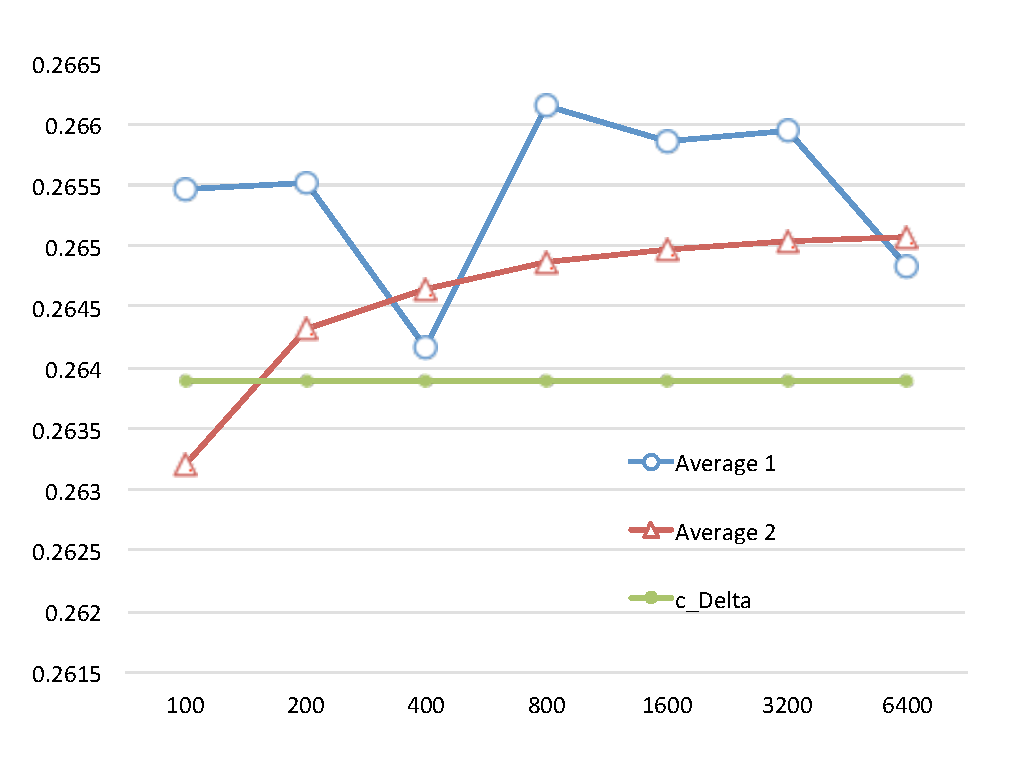
\includegraphics[width=12cm,bb=0 0 500 400]{numeresult1.pdf}
\caption{Average} \label{fig1}
\end{center}
\end{figure} 

\begin{figure}
\begin{center}
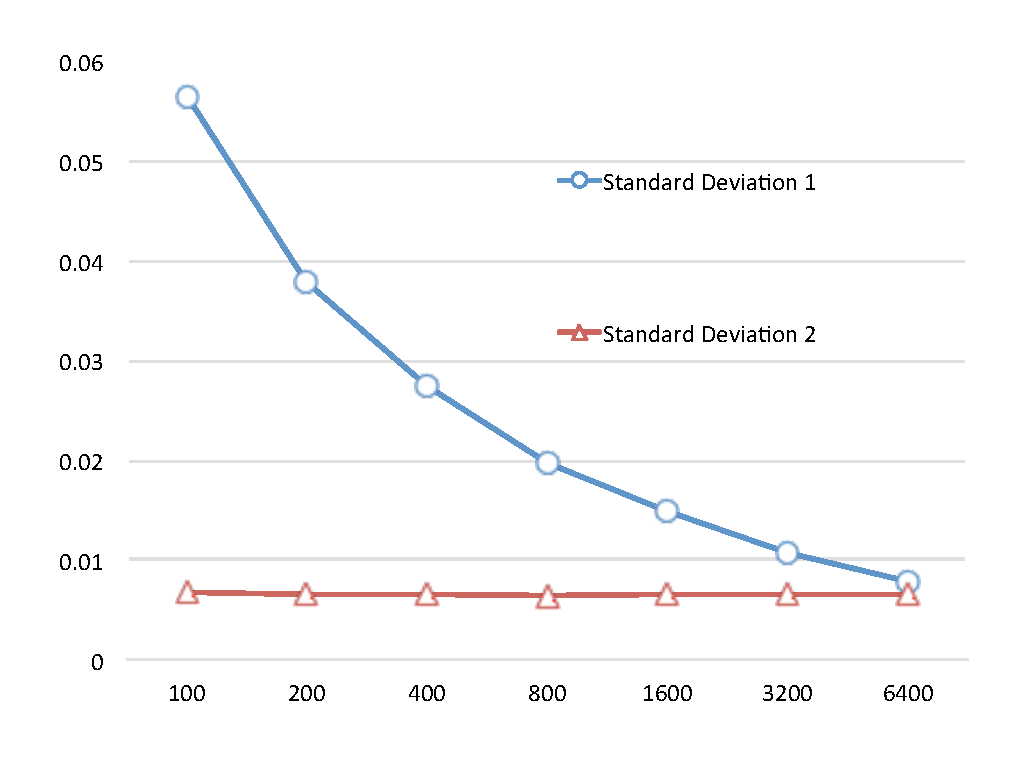
\includegraphics[width=12cm,bb=0 0 500 400]{numeresult2.pdf}
\caption{Standard Deviation} \label{fig2}
\end{center}
\end{figure} 

\subsection{Fx forward}
Here we calculate more realistic case.
Let $X$ be a process defined by the following SDE.
\begin{align}
  X(t) = x \exp\left( (\mu - \frac{1}{2} \sigma^2 )t + \sigma B(t)  \right).
\end{align}
\begin{align}
  c = E\left[\int_0^T  \left(V(X(T_i)) \vee 0 \right) dt \ \right], \\
  V(X(t)) = E\left[\ \sum_{T_i>t}F(X(T_i)) \ | \mathcal{F}_t \right]
\end{align}
\begin{center}
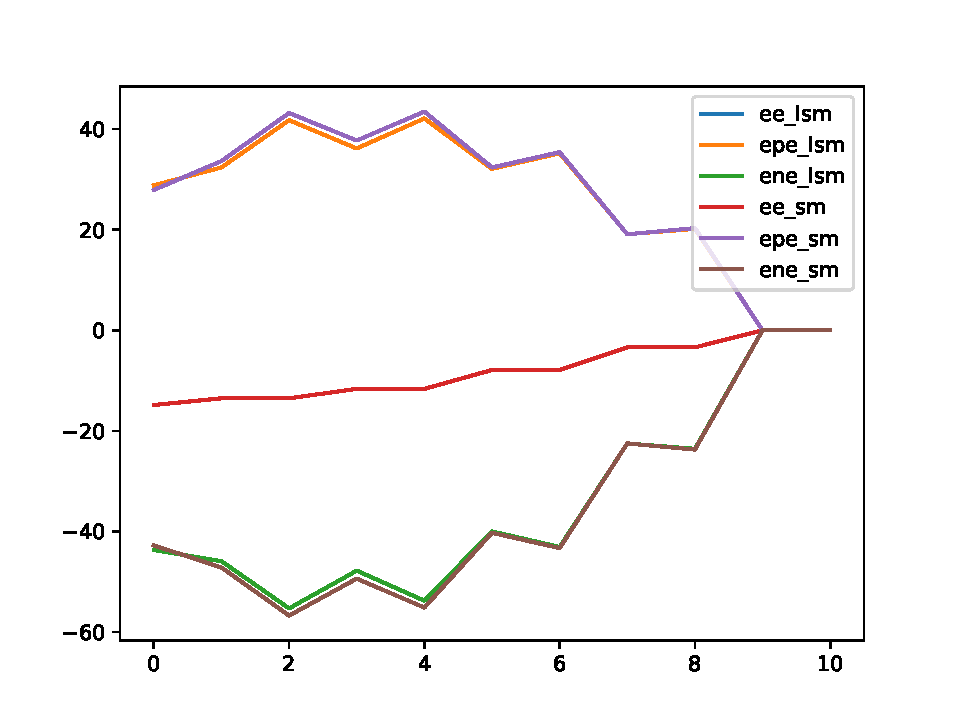
\includegraphics[width=10cm]{figure_1.pdf}
\end{center}
\begin{thebibliography}{99}

\bibitem{KM}Kusuoka, S. , and Y. Morimoto, 
\newblock Stochastic mesh methods for H{\" o}rmander type diffusion processes, 
\newblock Preprint.
%%
\bibitem{AH}Avramidis, A.N. , and P. Hyden, 
\newblock Efficiency improvements for pricing American options 
with a stochastic mesh, 
\newblock in Proceedings of the 1999 Winter Simulation Conference, pp. 344-350
%%
\bibitem{DU} Duffie, D., M. Huang, 1996,
\newblock  Swap Rates and Credit Quality, 
\newblock Journal of Finance, Vol. 51, No. 3, 921
%%
\bibitem{B} Belomestny, D., 
\newblock Pricing Bermudan Options by Nonparametric Regression: 
Optimal Rates of Convergence for Lower Estimates,
\newblock Finance and Stochastics, 15(2011), 655- 683.
%%
\bibitem{BG1} Broadie, M., and P. Glasserman,
\newblock A stochastic mesh method for pricing high-dimensional American options
\newblock J. Computational Finance, 7 (4) (2004), 35-72.
%
\bibitem{G}  Glasserman, P.,
\newblock "Monte Carlo Methods in Financial Engineering"
\newblock Springer,  2004, Berlin. 
%%
\bibitem{K}Kusuoka, S.,
\newblock Malliavin Calculus Revisited,
\newblock  J. Math. Sci. Univ. Tokyo 10(2003), 261-277.
%
\bibitem{KS2}Kusuoka, S., and D.W.Stroock, 
\newblock Applications of Malliavin Calculus II,
\newblock J. Fac. Sci. Univ. Tokyo Sect. IA Math. 32(1985),1-76.
%
\bibitem{LH} Liu, G., and L.J. Hong,
\newblock Revisit of stochastic mesh method for pricing American options,
\newblock Operations Research Letters 37(2009), 411-414.
%
\bibitem{Sh}Shigekawa, I.,
\newblock "Stochastic Analysis",
\newblock Translation of Mathematical Monographs vol.224,
AMS 2000.
%
\end{thebibliography}

\end{document}

